\section{Design}
% Section Overview
Having completed the analysis phase, we proceed to the design phase.
This stage specifies all key details needed for the implementation phase, ensuring that the system can be built precisely, efficiently, and with maintainability in mind. Object-Oriented Design (OOD) plays an essential role in this stage, as it enables the system to be structured into modular and reusable components, and helps preventing common pitfalls in product design such as \textit{design by guessing}, greatly reducing the necessary TTP (time-to-prototype), and consequently the TTM (time-to-market).

We dive into the system's core subsystems, namely the main server, the worker thread pool, the message routing mechanism, the authentication manager, and the database engine.
We aim to produce a set of UML diagrams, flowcharts, sequence diagrams, and pseudo-code that collectively serve as the blueprint for the implementation phase.

\subsection{Hardware Specification} % mostly done, need to paste
    % 4.1.1 Component Selection & Justification
    % 4.1.2 Raspberry Pi 4 Model B Specifications
    % 4.1.3 RGB LED Driver Circuit
    % 4.1.4 Power Supply & UPS Consideration
    % 4.1.5 Hardware Connection Diagram

% - Specify GPIO pins for LED (e.g., GPIO17, GPIO27, GPIO22 for R/G/B)
% - Calculate LED current limiting resistors (typically 220Ω-470Ω)
% - Document power requirements (Pi 4: 5V 3A minimum + LED overhead)
% - Create Fritzing/KiCAD wiring diagram
% - Justify Pi 4 choice (RAM for concurrent connections, GPIO availability)

\subsubsection{Component Selection}
% Raspberry Pi 4 specs, LED circuit, power supply
\subsubsection*{Raspberry Pi 4 Model B}

\par Since the project is intended to run on a compact and energy-efficient platform while supporting concurrent network connections, the Raspberry Pi 4 provides a good platform, thanks to its versatility, extensive community support, and compatibility with standard networking protocols make it well-suited for embedded server applications such as a multi-threaded chat system.

\begin{itemize}
    \item \textbf{Specifications}
    \begin{itemize}
        \item \textbf{CPU(SoC)}: Broadcom BCM2711, Quad-core Cortex-A72 (ARM v8) 64-bit 1.8GHz;
        
        \item \textbf{Memory}: 1GB, 2GB, 4GB or 8GB LPDDR4-3200;

        \item \textbf{Storage}: MicroSD card(operating system and data storage);

        \item \textbf{Connectivity}:
        \begin{itemize}
            \item 2 USB 3.0 ports;
            \item 2 USB 2.0 ports;
            \item 2 × micro-HDMI ports (4k60Hz supported);
        \end{itemize}

        \item \textbf{Networking}: 
        \begin{itemize}
            \item 2.4 GHz and 5.0 GHz IEEE 802.11ac wireless;
            \item Bluetooth 5.0, BLE;
            \item Gigabit Ethernet;
        \end{itemize}

        \item \textbf{GPU, Graphics and Display}:
        \begin{itemize}
            \item VideoCore VI (integrated into the BCM2711 SoC);
            \item OpenGL ES 3.1, Vulkan 1.0;
            \item Support for dual displays up to 4K resolution;
        \end{itemize}

        \item \textbf{GPIO}: Standard 40-pin GPIO header;

        \item \textbf{Input Power}: 
        \begin{itemize}
            \item 5V DC via USB-C connector (minimum 3A);
            \item 5V DC via GPIO header (minimum 3A);
            \item Power over Ethernet (PoE) enabled (requires separate PoE HAT);
        \end{itemize}

        \item \textbf{Dimensions}: 85mm(Length)  x 56mm(Width) x 17mm(Height);
    \end{itemize}
\end{itemize}


\begin{figure}[H]
    \centering
    \includegraphics[width=0.5\linewidth]{images/raspberry pi 4 model b.jpg}
    \caption{Raspberry Pi 4 Model B}
    \label{fig:raspberry_image}
\end{figure}

\bigskip

\subsubsection*{RGB LED}
\par An RGB LED (Red–Green–Blue Light Emitting Diode) is a single electronic component capable of producing a wide range of colors by combining light intensities from its three primary color elements.
Each color channel (red, green, and blue) can be independently controlled through pulse-width modulation (PWM) or simple digital output signals, allowing the LED to display different color states that correspond to various system conditions.

\par In this project, the RGB LED is connected to the Raspberry Pi's GPIO interface and serves as a visual status indicator for the server.
It provides immediate, low-power feedback about the system's operational state.
This makes it a practical and efficient diagnostic tool, especially since the Raspberry Pi server is intended to operate without a dedicated display or user interface.

\subsubsection*{Specifications}

\begin{itemize}
    \item Operating Voltage (per channel): 5V;
    \item Typical Foward Voltage (\(V_F\)):
    \begin{itemize}
        \item Red LED: 1.8$\sim$2.4V; 
        \item Green LED: 2.8$\sim$3.6V; 
        \item Blue LED: 2.8$\sim$3.6V;
    \end{itemize}
    \item Recommended LED Current: $\approx$ 20mA per channel;

    \item Common Anode;
    
    \item Total Power Consumption: 0.30W (with 0.05W margin);
\end{itemize}

\par Based on the estimated power consumption on the RGB LED, the Raspberry Pi 4 board power isn't meaningfully affected to require the need for a higher power/current power supply for the system.

\begin{figure}[H]
    \centering
    \includegraphics[width=0.2\linewidth]{images/RGB LED CA.png}
    \caption{RGB LED}
    \label{fig:rgb_led}
\end{figure}

\bigskip

\subsubsection*{LED Driver Transistor}
\par To interface the Raspberry Pi 4's 3.3 V GPIO outputs with the 5 V-powered RGB LED, each color channel requires a dedicated driver stage to ensure proper current handling and voltage compatibility. The driver provides electrical isolation between the Raspberry Pi's low-voltage control signals and the higher-voltage LED circuit, allowing safe and reliable switching of each color channel without exceeding the GPIO current limits.
\par The selected device, the BC547, is a general-purpose NPN (common anode) transistor widely used in low-power switching and amplification circuits. It is well-suited for this application due to it being inexpensive, broadly available and having optimal characteristics:

\begin{enumerate}
    \item \underline{Max collector current (\(I_{c,max}\)) = 100mA} : more than enough headroom as each LED will be needing around 20 mA per channel, making the circuit very stable and reliable;

    \item \underline{Collector–Emitter Saturation Voltage (\(V_{CE,sat}\)) = 0.2-0.3V}: low power loss when operating as a switch;

    \item \underline{High DC Current Gain (\(h_{FE}\)) = 100-800} : this high gain ensures that only a sub-milliampere current is required at the base to drive the transistor into saturation (fully "on"), allowing it to switch the 16 mA load. This minimal base current is easily supplied by the Pi's 3.3V GPIO pin through a suitable base resistor.
\end{enumerate}

\begin{figure}[H]
    \centering
    \includegraphics[width=0.25\linewidth]{images/BC547.png}
    \caption{BC547 Transistor}
\end{figure}

\subsubsection*{LED and Driver Resistors}
\par Each RGB channel is driven by a BC547 transistor, requiring one base resistor per transistor and one current-limiting resistor per LED channel. The current-limiting resistors are connected in series with the red, green, and blue LED channels to control the operating current, while the base resistors are connected in series with the transistor base terminals to limit the GPIO output current.
\par In total, six resistors are used in the circuit, three for the LEDs and three for the transistor bases. 

\par Starting with the base resistors:
\begin{itemize}
    \item \(I_C = I_{LED} \approx 20\,mA\)
    \item \(h_{FE,sat} = 15 \)
    \item \(V_{GPIO} = 3.3V\)
    \item \(V_{BE,sat} = 0.7V\)
\end{itemize}
\[
    I_B = I_C/h_{FE,sat} = 1.3 \,mA
\]
\[
R_B = (V_{GPIO} - V_{BE,sat})/I_B  \approx 2k\Omega
\]

\bigskip

\par Now the LED current limiting resistors:
\begin{itemize}
    \item \(V_{S} = 5V\)
    \item \(V_{CE,sat} \approx 0.15V\)
    \item \(V_{F_{RED}} \approx 2.1V\)
    \item \(V_{F_{GREEN,BLUE}} \approx 3.2V\)
\end{itemize}
\[
    R_{C_{RED}} = (V_{S} - V_{CE,sat} - V_{F_{RED}})/I_C  \approx  140\Omega
\]

\[
    R_{C_{GREEN,BLUE}} = (V_{S} - V_{CE,sat} - V_{F_{GREEN,BLUE}})/I_C  \approx  80\Omega
\]

\bigskip

\subsubsection*{Power Supply Unit}
\par The system operates from a regulated 5 V DC input supplied through the Raspberry Pi 4's USB-C connector. According to the official datasheet, a 5 V / 3 A power source is sufficient, provided that attached USB peripherals draw less than 500 mA in total. This configuration meets the project's requirements, as the only additional load is the RGB status LED, which consumes approximately 30 mA (0.15 W).
\par A stable power source is essential to maintain consistent performance and prevent voltage drops that could lead to instability, unexpected shutdowns, or database corruption. To improve reliability, the design includes an optional Uninterruptible Power Supply (UPS) that provides short-term backup power and allows the system to perform a controlled shutdown in case of an extended outage. This safeguard ensures data integrity for the active SQLite database and supports graceful server termination.

\subsubsection{Hardware Connection Diagram}
% Wiring diagram showing Pi → LED, Pi → Network, Pi → Power
\par The hardware connections for this project are straightforward and primarily consist of the GPIO interfaces linked to the RGB LED driver circuit. An equally important aspect is the system's power connection, which supplies regulated 5 V DC to the Raspberry Pi and associated components. As discussed previously, this power connection can optionally include an uninterruptible power supply (UPS) to enhance system reliability and ensure data integrity during power interruptions.

\subsubsection*{General Hardware Connection}
\begin{figure}[H]
    \centering
    \includegraphics[width=0.65\linewidth]{images/Hardware Connections.drawio.png}
    \caption{General Hardware Connection.}
    \label{fig:connections}
\end{figure}

\subsubsection*{GPIO-RGB LED Connection}

\begin{figure}[H]
    \centering
    \includegraphics[width=0.8\linewidth]{images/RGB LED GPIO Connections.drawio.png}
    \caption{GPIO connections to the Transistor LED Drivers.}
    \label{fig:transistor_connections}
\end{figure}

\begin{figure}[H]
    \centering
    \includegraphics[width=0.45\linewidth]{images/GPIO_rasp_pins.png}
    \caption{GPIO pin layout on the Raspberry Pi 4 Model B.}
    \label{fig:rasp_pins}
\end{figure}

\par The GPIO pins GPIO17, GPIO22, and GPIO27 were selected to control the red, green, and blue channels of the RGB LED, respectively. These pins were chosen because they are general-purpose I/O lines without predefined alternate functions that could interfere with other possible system peripherals. They are all located on the same side of the Raspberry Pi's GPIO header, which simplifies wiring and layout on a breadboard or PCB. Furthermore, these pins support standard 3.3 V logic levels and can safely source or sink the small control currents required by the transistor base resistors, making them well suited for driving the LED channels.

\subsection{Software Architecture} 
\subsubsection{Development Tools}
% Buildroot, GCC ARM cross-compiler, VS Code
The development environment comprises two main tools: 

\begin{itemize}
    \item \textbf{Buildroot:} Used to generate the embedded Linux image and integrate all required libraries, frameworks, and toolchain components. 
    \item \textbf{Visual Studio Code (VS Code):} Integrated development environment for application coding, debugging, and version control.
\end{itemize}

Buildroot provides the cross-compilation toolchain, specifically the \texttt{aarch64-linux-g++} compiler, enabling native binaries to be built on the host and easily deployed to the Raspberry Pi target.

The choice of VS Code is motivated by its ecosystem integration and ease of automation:
\begin{itemize}
    \item \textbf{Git integration:} Native version control allows synchronized collaboration and incremental updates between the two group members.
    \item \textbf{Makefile support:} Combined with SSH key-based authentication between host and target, the build process supports remote cross-compilation and direct deployment of specific modules for rapid functional validation.
\end{itemize}

\subsubsection{Libraries and Frameworks}
\textbf{SQLite}

\begin{figure}[H]
    \centering
    \includegraphics[width=0.3\linewidth]{images/SQLite.png}
    \caption{SQLite: Embedded database engine}
    \label{fig:sqlite_logo}
\end{figure}

SQLite is a self-contained, serverless, zero-configuration SQL database engine. For Huxley, SQLite provides:

\begin{itemize}
    \item \textbf{WAL Mode:} Write-Ahead Logging enables concurrent reads during writes; critical for 25 simultaneous client authentications
    \item \textbf{Prepared Statements:} Prevents SQL injection attacks via parameterized queries
    \item \textbf{Zero Administration:} No separate server process; database is a single file on the microSD card
    \item \textbf{ACID Guarantees:} Atomic commits ensure message persistence survives power loss
\end{itemize}
%% For more information on design principles:
% https://en.wikipedia.org/wiki/ACID
% ACID is a set of four properties—atomicity, consistency, isolation, and durability—that guarantee the reliability of database transactions, ensuring data remains valid even in the event of errors or system failures


\vspace{0.5cm}
\textbf{libsodium 1.0.20}
\begin{figure}[H]
    \centering
    \includegraphics[width=0.5\linewidth]{images/libsodium.png}
    \caption{libsodium: Modern cryptographic library}
    \label{fig:libsodium_image}
\end{figure}

Libsodium provides production-grade cryptographic primitives for Huxley:
\begin{itemize}
    \item \textbf{Password Hashing:} \texttt{crypto\_pwhash} implements Argon2id
    \item \textbf{Message Encryption:} \texttt{crypto\_secretbox} provides authenticated encryption (XSalsa20 + Poly1305 MAC)
    \item \textbf{Key Derivation:} Automatic salt generation, configurable work factors (memory + CPU cost)
    \item \textbf{Constant-Time Operations:} Prevents timing attacks during password verification
\end{itemize}

\vspace{0.5cm}

\textbf{PThreads} \\
POSIX threads provide lightweight concurrency and allows us to create a worker pool. Each worker thread multiplexes multiple clients using epoll (see \texttt{man epoll (7)} for more information), sharing access to AuthManager and MessageRouter, in some cases via mutex-protected sections.
\textbf{Key Primitives Used:}
\begin{itemize}
    \item \texttt{pthread\_create()}: Spawn fixed worker pool at startup
    \item \texttt{pthread\_join()}: Graceful shutdown—wait for workers to terminate
    \item \texttt{pthread\_mutex\_t}: Protect activeClients map, socketQueue
\end{itemize}

\subsubsection*{Buildroot Settings}
% Images and settings to enable the libraries and frameworks
\begin{figure}[H]
    \centering
    \includegraphics[width=0.5\linewidth]{images/Target-Architecture.png}
    \caption{Buildroot: Target Architecture}
\end{figure}
We set the target architecture as AArch64 (little endian) with the variant for the cortex-A72. MMU-page size is kept to the default value of 4Kb. The root filesystem was configured as ext4 to support SQLite persistence.
\begin{figure}[H]
    \centering
    \includegraphics[width=0.5\linewidth]{images/Toolchain.png}
    \caption{Buildroot: Toolchain}
\end{figure}
In the toolchain options, we select the glibc C library, and enable support for C++. 

\begin{figure}[H]
    \centering
    \includegraphics[width=1\linewidth]{images/Debugging tools and OpenSSH.jpeg}
    \caption{Buildroot: OpenSSH, gdb, Valgrind}
\end{figure}
During implementation, we selected three important libraries, to be used for connection and deployment of the application (OpenSSH), as well as to provide tests, debugging (gdb) and profiling features (Valgrind).

\begin{figure}[H]
    \centering
    \includegraphics[width=0.2\linewidth]{images/dhcpcd.png}
    \caption{Buildroot: dhcpcd}
\end{figure}
The ISC DHCP server (dhcpcd) is included among the core network utilities. It assigns static IP leases to ensure consistent addressing between the Raspberry Pi and development hosts, simplifying SSH access and multi-client testing.

\begin{figure}[H]
    \centering
    \includegraphics[width=\linewidth]{images/Libraries.jpeg}
    \caption{Buildroot: libsodium, sqlite, json-for-modern-cpp}
\end{figure}
In the libraries section, we select libsodium (all functions), json-for-modern-cpp, and sqlite with "convenient access to metadata about tables and queries". 

The final Linux image, with the debugging tools plus a few extras (such as vim and other quality-of-life tools), is $159.4$MB. 

% Package Diagram subsection 
\subsection{Package-level Design}
    % 4.8.1 Package Diagram
    % 4.8.2 Package Descriptions
The package-level design gives a high-level, hierarchical overview of the system. It organises and separates it into modular components, each responsible for a specific aspect of the application's functionality. It also tells us how these components are communicating with each other. 

Figure~\ref{fig:package_diagram} illustrates the package structure of the messaging application.
\begin{figure}[H]
    \centering
    \includegraphics[width=\textwidth]{images/design-Package_Diagram.png}
    \caption{Package-level design diagram}
    \label{fig:package_diagram}
\end{figure}

%%% What it should contain: 
%% Client side 
% Basic UI, client protocol handler, and network layer
%% Server side (all of the aforementioned design components)
% Network layer, protocol handler, authentication manager, message router, database access layer, cryptography engine, logging module, and utility functions.
%% 

% Let's try to keep this high-level, short, and not too implementation-biased.
\subsubsection{Package Descriptions}
\textbf{Client Application Package:}
\begin{itemize}
    \item \textbf{UI Module:} Manages user interface components, including login
    \item \textbf{Client Protocol Handler:} Implements client-side protocol framing and JSON serialization/deserialization
    \item \textbf{Network Module:} Manages network connections and communication with the server
\end{itemize}
% keep testing and utils out
\textbf{Server Application Package:}
\begin{itemize}
    \item \textbf{Network Module:} Handles TCP socket management, epoll-based
    \item \textbf{Protocol Handler:} Parses incoming frames, constructs outgoing frames
    \item \textbf{Authentication Manager:} Manages user registration, login, and
    \item \textbf{Message Router:} Routes messages between clients, manages delivery status
    \item \textbf{Database Access Layer:} Abstracts SQLite operations, prepared statements
    \item \textbf{Cryptography Engine:} Provides password hashing and message encryption
    \item \textbf{Logging Module:} Records security-relevant events to the database
    \item \textbf{Configuration Module:} Loads and manages server configuration parameters
\end{itemize}

\subsection{Class Architecture}
% 4.3 Class Diagram & Architecture
%     4.3.1 Class Diagram (UML) DONE
%     4.3.2 Class Descriptions DONE
%         - Huxley Server 
%         - WorkerThread
%         - ClientState
%         - ProtocolHandler
%         - Command 
%         - AuthManager
%         - MessageRouter
%         - Database
%         - CrpytoEngine
%         - StatusManager

\subsubsection{Class Diagram}
The class diagram forms the basis for the software implementation to be developed in the next phase.
Figure~\ref{fig:class_diagram} shows the system's object-oriented design (OOD) with clear separation of concerns: server, worker pool, authentication, message routing, database access, protocol handling, and lastly, status indication through the LED. 

\begin{figure}[H]
    \centering
    \includegraphics[width=\textwidth]{images/design-ClassDiagram.png}
    \caption{UML Class Diagram. Two layers are emphasized: concurrency and service.}
    \label{fig:class_diagram}
\end{figure}

\subsubsection{Class Descriptions}
The system follows SOLID principles: each class has a single, well-defined responsibility, depends on abstractions (Database interface), and components are loosely coupled through dependency injection.

The SOLID principles are as follows: 
\begin{itemize}
    \item \textbf{S - Single Responsibility:} every class should encapsulate a single, well-defined responsibility. 
    \item \textbf{O - Open/Closed:} Open for extension, Closed for modification - this means you should be able to add new behaviour without altering the existing code.
    \item \textbf{L - Liskov Substitution:} every subclass can be used where the parent is expected, as everything is still expected to behave correctly.
    \item \textbf{I - Interface Segregation:} clients (instances) shouldn't be forced to depend on interfaces they don't use. 
    \item \textbf{D - Dependency Inversion:} have the details (implementation) adapt to the high-level abstractions, not the opposite.    
\end{itemize}

Our main focus for the server are all but L, given we have no subclasses. Our goal for this section is then to provide a thorough exposition of the classes, separating functionalities, and making sure implementation doens't guide abstraction, but the other way around. 

\textbf{HuxleyServer}
\begin{itemize}
    \item \textbf{Responsibility:} Main orchestrator—owns worker thread pool, socket queue, and shared subsystems (AuthManager, MessageRouter, Database). Producer role
    \item \textbf{Key Attributes:}
        \begin{itemize}
            \item \texttt{workerThreads}: fixed pool of WorkerThread instances
            \item \texttt{socketQueue}: queue of file descriptors of accepted client
            \item \texttt{queueMutex}: queue synchronization
        \end{itemize}
    \item \textbf{Key Methods:}
        \begin{itemize}
            \item \texttt{start(port)}: Initialize database, spawn worker pool, bind socket, enter accept loop
            \item \texttt{acceptLoop()}: Block on accept(), push client\_fd to socketQueue
            \item \texttt{stop()}: Set global shutdown flag, join all worker threads, cleanup resources
        \end{itemize}
    \item \textbf{SOLID:} Single Responsibility (orchestration only), Open/Closed (workers are polymorphic)
\end{itemize}

\textbf{WorkerThread}
\begin{itemize}
    \item \textbf{Responsibility:} Event-driven I/O multiplexing, handles multiple clients via epoll, dispatch commands to service layer. Consumer role
    \item \textbf{Key Attributes:}
        \begin{itemize}
            \item \texttt{epollFd}: File descriptor for the worker's private epoll instance used by the event loop; not shared across threads. 
            % Monitors client sockets and the wakeupFd to notify the worker of new assignments or I/O events.
            \item \texttt{wakeupFd}: File descriptor to interrupt epoll\_wait() from main thread, written to whenever handing over new clients
            \item \texttt{clientStates}: Map of \texttt{socket\_fd → ClientState*} tracking per-connection state
        \end{itemize}
    \item \textbf{Key Methods:}
        \begin{itemize}
            \item \texttt{run()}: thread function, loop—epoll\_wait(), process ready events
            \item \texttt{notifyEvent(fd)}: triggered when there's a new addition to the outgoing message queue of a client
            \item \texttt{handleReadEvent(fd)}: Read bytes into ClientState.recvBuffer, parse with parseCommand(), call processCommand()
            \item \texttt{handleWriteEvent(fd)}: Flush ClientState.sendQueue to socket, disable EPOLLOUT if empty, call processCommand()
            \item \texttt{processCommand(state, cmd)}: Authorization check, dispatch to AuthManager or MessageRouter based on command type
        \end{itemize}
    \item \textbf{SOLID:} Single Responsibility (I/O only, no business logic), Dependency Inversion (uses AuthManager/MessageRouter abstractions)
\end{itemize}

\textbf{ClientState}
\begin{itemize}
    \item \textbf{Responsibility:} Tracks session state per client
    \item \textbf{Key Attributes:}
        \begin{itemize}
            \item \texttt{owner}: points to the parent worker thread responsible for the socket. Used to notify owner when new event enters the \texttt{sendQueue}
            \item \texttt{socketFd}: client's TCP socket file descriptor
            \item \texttt{username}: authenticated user identifier (empty string if unauthenticated)
            \item \texttt{authenticated}: boolean flag checked before allowing privileged commands
            \item \texttt{lastActivity:} stores the last time an activity was issued to/from the socket
            \item \texttt{recvBuffer}: incoming data is buffered until a complete JSON message is received
            \item \texttt{sendQueue}: (bounded) queue of outgoing JSON responses
        \end{itemize}
    \item \textbf{Key Methods:}
        \begin{itemize}
            \item \texttt{isAuthenticated()}: Returns \texttt{authenticated} flag—used for authorization checks
            \item \texttt{queueResponse(msg)}: Push serialized JSON to sendQueue, call notifyEvent
        \end{itemize}
    \item \textbf{SOLID:} Single Responsibility (state management only), Interface Segregation (minimal public API)
\end{itemize}

% TODO Question here on the "result". Is it an extension of "Command"? We have the "Command" struct. Should we add result as the union of that with an error struct?
\textbf{ProtocolHandler}
\begin{itemize}
    \item \textbf{Responsibility:} Protocol translation layer—serialize/deserialize JSON messages
    \item \textbf{Key Methods:}
        \begin{itemize}
            \item \texttt{parseCommand(json)}: Parse JSON string into Command struct (type, username, password, recipient, content fields)
            \item \texttt{serializeResponse(result)}: Convert operation result into JSON response (success/error codes, data payload)
        \end{itemize}
    \item \textbf{SOLID:} Single Responsibility (protocol encoding/decoding), Open/Closed (can extend with new command types without modifying existing code)
\end{itemize}

% \textbf{Command}
% \begin{itemize}
%     \item \textbf{Responsibility:} Data Transfer Object—immutable command representation
%     \item \textbf{Key Attributes:}
%         \begin{itemize}
%             \item \texttt{type}: CommandType enum (LOGIN, REGISTER, SEND\_MESSAGE, LOGOUT)
%             \item \texttt{username, password, recipient, content}: Command-specific data fields
%         \end{itemize}
%     \item \textbf{SOLID:} Single Responsibility (data container), Liskov Substitution (polymorphic command handling)
% \end{itemize}

\textbf{AuthManager}
\begin{itemize}
    \item \textbf{Responsibility:} Authentication logic—password hashing, verifies credentials 
    \item \textbf{Key Methods:}
        \begin{itemize}
            \item \texttt{registerUser(username, password)}: Hash password with Argon2id, call \texttt{database→insertUser()}
            \item \texttt{loginUser(username, password)}: Retrieve stored hash via \texttt{database→findUser()}, verify with \textbf{constant-time comparison}
            \item \texttt{hashPassword(password)}: Private helper—generates salt, applies Argon2id (parameters set in \texttt{Config} Entity)
        \end{itemize}
    \item \textbf{SOLID:} Single Responsibility (authentication only), Dependency Inversion (depends on Database abstraction, not concrete SQLite)
\end{itemize}

\textbf{MessageRouter}
\begin{itemize}
    \item \textbf{Responsibility:} Message delivery logic—route to online clients or queue for offline delivery
    \item \textbf{Key Attributes:}
        \begin{itemize}
            \item \texttt{activeClients}: Map of \texttt{username → ClientState*} (protected by clientsMutex)
            \item \texttt{clientsMutex}: Pthread mutex serializing access to activeClients
        \end{itemize}
    \item \textbf{Key Methods:}
        \begin{itemize}
            \item \texttt{registerClient(username, state)}: Lock mutex, insert into activeClients map (called after successful login)
            \item \texttt{unregisterClient(username)}: Lock mutex, erase from activeClients (called on logout/disconnect)
            \item \texttt{routeMessage(sender, recipient, content)}: Encrypt via cryptoEngine, persist to database with \texttt{delivered=0}, check activeClients—if online, queue in recipient's sendQueue
        \end{itemize}
    \item \textbf{SOLID:} Single Responsibility (routing logic), Dependency Inversion (depends on Database/CryptoEngine abstractions)
\end{itemize}

\textbf{Database}
\begin{itemize}
    \item \textbf{Responsibility:} Data persistence layer—SQLite interface with prepared statements
    \item \textbf{Key Attributes:}
        \begin{itemize}
            \item \texttt{dbHandle}: SQLite3 connection handle (WAL mode enabled)
        \end{itemize}
    \item \textbf{Key Methods:}
        \begin{itemize}
            \item \texttt{insertUser(username, hash)}: Prepared statement prevents SQL injection—bind parameters, execute INSERT
            \item \texttt{findUser(username, outHash)}: Retrieve password\_hash for authentication (indexed lookup)
            \item \texttt{insertMessage(sender\_id, recipient\_id, encrypted)}: Store encrypted message with \texttt{delivered=0}
            \item \texttt{getQueuedMessages(recipient\_id)}: Query messages WHERE \texttt{recipient\_id=? AND delivered=0} (indexed)
            \item \texttt{markDelivered(message\_id)}: UPDATE messages SET \texttt{delivered=1} WHERE \texttt{id=?}
            \item \texttt{logActivity(log)}: INSERT INTO logs with automatic timestamp
        \end{itemize}
    \item \textbf{SOLID:} Single Responsibility (data access only), Interface Segregation (could define IDatabase interface for testing)
\end{itemize}

\textbf{CryptoEngine}
\begin{itemize}
    \item \textbf{Responsibility:} Cryptographic operations—authenticated encryption/decryption
    \item \textbf{Key Methods:}
        \begin{itemize}
            \item \texttt{encryptMessage(plaintext)}: Generate random nonce, apply XSalsa20+Poly1305 (libsodium secretbox), return ciphertext with MAC
            \item \texttt{decryptMessage(cipher)}: Verify MAC, decrypt payload—reject if MAC invalid (prevents tampering)
        \end{itemize}
    \item \textbf{SOLID:} Single Responsibility (encryption only), Open/Closed (can swap crypto algorithms without changing callers)
\end{itemize}

\textbf{StatusManager}
\begin{itemize}
    \item \textbf{Responsibility:} Hardware abstraction layer—control RGB LED visual indicators
    \item \textbf{Key Methods:}
        \begin{itemize}
            \item \texttt{setLedColor(color)}: Write to GPIO pins to set LED state (GREEN=idle, YELLOW=processing, RED=error)
        \end{itemize}
    \item \textbf{SOLID:} Single Responsibility (hardware control), Dependency Inversion (could define IStatusIndicator interface for headless testing)
\end{itemize}

\subsection{Database Design}
% 4.2.2 Database Schema Design
%         - Entity definitions (Users, Messages, Logs)
%         - Relationships & Foreign Keys
%         - Indexes for performance
%         - WAL mode configuration
In this section, we define the Persistence Layer of our system. We identify which entities are contained in our database, and establish the relationships between them. 

\begin{figure}[H]
    \centering
    \includegraphics[width=0.8\linewidth]{images/design-Logical_Database_Design.png}
    \caption{Logical database schema illustrating entity relationships between users, messages, configuration parameters, and log records.}
    \label{fig:database_overview}
\end{figure}

The database layer defines the system's durable state. It provides transactional guarantees for user authentication, message delivery, and audit logging. Figure \ref{fig:database_overview} presents the logical schema, showing entity relationships and data dependencies.

\subsubsection{Schema Definition}
The database has four different entities:
\begin{itemize}
    \item Users; 
    \item Messages;
    \item Logs;
    \item Config;  
\end{itemize}
each optimized for concurrent access via SQLite's Write-Ahead Logging (WAL) mode. 

\textbf{Users} - Stores user account information:
        \begin{itemize}
            \item \texttt{UserID}: unique ID for each new user;
            \item \texttt{username}: user's username, and cannot be duplicated nor empty(NULL).
            \item \texttt{password\_hash}: the account's password hash, used for authentication, cannot be empty. 
            \item \texttt{created\_at}: user account creation date.
        \end{itemize}

\textbf{Messages table} - Stores encrypted private messages exchanged between users:
        \begin{itemize}
            \item \texttt{MessageID}: unique id for each message.
            \item \texttt{sender\_id}: ID of the user who sent the message.
            \item \texttt{recipient\_id}: ID of the user who received the message.
            \item \texttt{ciphertext, nonce, tag}: encrypted message data, required for decryption with secret key.
            \item \texttt{timestamp}: time when the message was sent.
            \item \texttt{delivered}: message delivery status (1=delivered or 0=not delivered).
        \end{itemize}
        
Both the sender\_id and recipient\_id refer to the Users table. These are 1..N relations from the UserID to both sender\_id and recipient\_id. This means that each user may send and receive an arbitrary (N) number of messages, not necessarily the same. 
Note that all text fields use UTF-8 encoding to ensure cross-platform compatibility.
Ciphertext, nonce, and tag are stored as BLOBs to preserve binary data without encoding overhead.
Indexing is used to check for undelivered messages, and to fetch for recent messages by time and sender.
    
\textbf{Logs table} - Stores user logs, for debugging or auditing purposes. Also useful for auditability and intrusion detection purposes.
        \begin{itemize}
            \item \texttt{LogID}: unique log entry ID.
            \item \texttt{level}: log message type. 
            \item \texttt{log}: log message text.
            \item \texttt{timestamp}: log event date.
        \end{itemize}

Logs are purged periodically to prevent SD-card wear; archival thresholds are configurable via the Config entity

\textbf{Config table} - stores system-wide parameters that must persist across reboots, including Argon2id hashing parameters and security versioning.
        \begin{itemize}
            \item \texttt{config\_id}: primary key for config.
            \item \texttt{memory\_param}: memory param, used in argon2id hashing. 
            \item \texttt{iteration\_param}: iteration param, used in argon2id hashing.
            \item \texttt{log\_purge}: number of logs to have before cleanup
        \end{itemize}

\subsubsection{WAL Mode Justification}
Write-Ahead Logging enables concurrent read operations during write transactions. When a client authenticates (read from \texttt{users} table) while another client sends a message (write to \texttt{messages} table), both operations proceed without blocking. This is critical for supporting 25 concurrent connections with sub-second authentication latency, and it ensures real-time responsiveness.

\subsubsection{Runtime Pragmas}
The system enforces \texttt{journal\_mode=WAL}, \texttt{synchronous=NORMAL}, and \texttt{foreign\_keys=ON}, and applies memory optimizations (\texttt{mmap\_size=256 MB}, \texttt{page\_size=4096}). These settings improve concurrent read/write throughput and reduce lookup latency.

\texttt{mmap\_size} enables direct memory mapping of up to 256 MB of the database file, eliminating read() syscalls (except the first) and leveraging the kernel’s page cache (the ARMv8-A MMU performs the actual virtual$\to$ physical translation; \texttt{page\_size=4096} aligns SQLite’s internal B-tree pages with the system’s 4 KB memory pages, minimizing fragmentation and improving I/O alignment on embedded flash storage.

\subsubsection{Indexing Strategy}
To reduce query latency and guarantee constant-time lookups under concurrent load, the following indexes are defined:
\begin{itemize}
    \item \texttt{idx\_username}: Accelerates user lookup during authentication (O(log n) vs O(n))
    \item \texttt{idx\_recipient\_delivered}: Optimizes queued message retrieval (WHERE recipient\_id=? AND delivered=0)
    \item \texttt{idx\_sender\_timestamp}: Enables efficient message history queries sorted by time
\end{itemize}
Index maintenance overhead is negligible compared to the performance gain in authentication and delivery queries.

\subsection{Task \& Thread Specification}
%% Thread Roles
% - Main Thread
% - Worker Threads
%% Event Dispatch
% epoll: monitor client sockets + wakeupFd
% events 
%% Synchronisation
% per-client state: requires locking 
% shared maps: active clients, protected by mutexes 
% assignment queues: wakeupFd interrutps epoll 
% Deadlock policy: strict lock order (clientsMutex < ledMutex)

\label{sec:threads}
\subsubsection{Thread Roles}
\par \textbf{Main Thread (acceptor/orchestrator).} Single producer of client sockets; owns process lifetime, bootstraps subsystems, selects a worker for each accepted connection, and drives shutdown.
\par \textbf{Worker Threads (I/O reactors).} Fixed-size pool one per CPU core). Each worker owns: (i) a private \texttt{epoll} instance, (ii) a \texttt{wakeupFd} (eventfd) registered in epoll, (iii) an assignment queue (bounded MPSC), and (iv) the per-connection state of all sockets assigned to it (clientState). No socket is shared across workers, as each socket is assigned to only one worker.

\begin{figure}[H]
    \centering
    \includegraphics[width=\textwidth]{images/design-Event_Poll_Architecture.png}
    \caption{Kernel-user event architecture: epoll red-black tree, ready list, and per-thread event loop interaction.}
    \label{fig:event_poll_arch}
\end{figure}

\paragraph{Invariants.}
\begin{itemize}
  \item \textbf{Exclusive socket ownership:} After assignment, \texttt{fd} is touched by its worker only.
  \item \textbf{Non-blocking I/O:} All sockets are \texttt{O\_NONBLOCK}; workers never call blocking primitives except \texttt{epoll\_wait()}.
  Notice it blocks the \textit{thread} not the CPU. 
  \item \textbf{One DB handle per worker:} Each worker holds its own SQLite connection; no connection reuse across threads.
\end{itemize}

\subsubsection{Initialization Sequence (Main Thread)}
\begin{enumerate}
  \item \textbf{Database.} Open SQLite file, set
  \texttt{PRAGMA journal\_mode=WAL; PRAGMA synchronous=NORMAL;}, create tables and indexes if absent.
  \item \textbf{Shared Services.} Construct \textit{AuthManager}, \textit{MessageRouter}, \textit{CryptoEngine}, \textit{StatusManager}.
  \item \textbf{Worker Pool.} Spawn $N=\text{num\_cores}$ workers; each creates \texttt{epollFd} and \texttt{wakeupFd} (added to epoll with \texttt{EPOLLIN}).
  \item \textbf{Listening Socket.} Create, \texttt{setsockopt(SO\_REUSEADDR|SO\_REUSEPORT)}, bind, listen; mark non-blocking.
\end{enumerate}

\subsubsection{Accept/Assignment Loop (Main Thread)}
The main thread's core functionality is, besides initialization, to accept new connections (or reject if full), and to service them to a given worker thread.
\begin{enumerate}
  \item \textbf{Accept.} Repeatedly call \texttt{accept4(..., SOCK\_NONBLOCK)}; on \texttt{EAGAIN}, back to wait (e.g., \texttt{poll} on the listening socket or simple loop if edge-driven by SO\_REUSEPORT).
  \item \textbf{Select Worker.} \emph{Least-loaded} by active-connection count (\textit{tiebreaker}: lowest worker id). Complexity $O(1)$ with a min-heap.
  \item \textbf{Enqueue.} Push \texttt{fd} into the worker's bounded queue (capacity $C$). On success, write \texttt{uint64\_t(1)} to the worker's \texttt{wakeupFd}. On overflow, reject with ``server busy'' and close \texttt{fd}.
\end{enumerate}

\begin{figure}[H]
    \centering
    \includegraphics[width=\linewidth]{images/design-MainThread_Flowchart.png}
    \caption{Main thread accept–assignment loop showing connection acceptance, worker selection, and queue signaling.}
    \label{fig:main_thread_flow}
\end{figure}

% Some questions that need to be answered: is the waken up thread the one servicing the new sockets in socketQueue? Popping them, that is? If so, we need to lock the queue. (Mutex checks out)
% And that is maintained with a priorityQueue whose predicate involves the size of each workerThread's clientStates map? 
\subsubsection{Worker Threads}
\begin{figure}[H]
    \centering
    \includegraphics[width=\linewidth]{images/design-Worker_Thread_Flowchart.png}
    \caption{Worker thread lifecycle and assignment handling loop.}
    \label{fig:worker_thread_flow}
\end{figure}

In this subsection, we outline the behavior and functioning of worker threads. Fig.\ref{fig:worker_thread_flow}
provides a high-level overview of the worker thread behaviour.
\paragraph{Startup.}
Create \texttt{epollFd}, \texttt{wakeupFd}; register \texttt{wakeupFd} with \texttt{EPOLLIN}. Open per-thread SQLite handle (WAL)
Each worker thread waits on the \texttt{epoll\_wait}, until waken up to register new sockets, or to receive events from already registered ones. 

\begin{figure}[H]
    \centering
    \includegraphics[width=\textwidth]{images/design-Event_Poll_Flow.png}
    \caption{Worker thread lifecycle showing accept, dispatch, read/write event handling.}
    \label{fig:event_poll_flow}
\end{figure}

\paragraph{Assignment Drain}
For each new \texttt{fd} that is popped from the queue: set it as \texttt{O\_NONBLOCK}, allocate a new \texttt{ClientState} instance to monitor it, and register in epoll with \texttt{EPOLLIN}. Insert into \texttt{clientStates[fd]}. The worker thread is now monitoring the socket, and has the necessary information stored in ClientState to use servicing logic from the service abstraction classes (\textit{AuthManager}, and \textit{MessageRouter}).

\paragraph{Read Event (length-prefixed JSON)}
Accumulate bytes into the client's \texttt{state.recvBuffer}. If \texttt{recvBuffer.size() \textgreater= 4} and a full frame is present:
\begin{enumerate}
  \item Parse one complete frame; on malformed JSON $\rightarrow$ send \texttt{400} error and optionally close.
  \item Dispatch: \emph{LOGIN/REGISTER} $\rightarrow$ \textit{AuthManager}; \emph{SEND\_MESSAGE} $\rightarrow$ \textit{MessageRouter}.
  \item Update \texttt{state.lastActivity = now()}. % where is this state? is this necessary for timeout reasons? 
\end{enumerate}
% Too much implementation bias: \emph{Edge-triggered note:} When using \texttt{EPOLLET}, continue \texttt{recv()} until it returns \texttt{-1/EAGAIN}.
\textbf{Outbound queue safety:} ClientState owns a pthread\_mutex\_t sendMutex protecting sendQueue. Producers (e.g., MessageRouter) lock, push, unlock, then notify via notifyEvent. The worker locks briefly to pop before flushing. Critical sections are short and contention sparse.

\paragraph{Write Event}
While sendQueue is non-empty, issue send() on the front frame; on partial write keep EPOLLOUT enabled; when the queue becomes empty, epoll\_ctl(… drop EPOLLOUT).
Delivery flag: set delivered=1 when the frame for recipient has been fully written to the kernel (transport-level).

\paragraph{Event Handling Flowcharts}
Figures~\ref{fig:inbound_event_flow}–\ref{fig:disconnect_event_flow} illustrate the per-worker
event dispatch logic for each epoll-triggered event type. These complement the
reactor semantics described earlier, aiming for thread isolation and ensuring
message delivery.

\begin{figure}[H]
  \centering
  \includegraphics[width=\textwidth]{images/design-InboundEvent.png}
  \caption{Inbound event handling flow (EPOLLIN): message parsing and authentication.}
  \label{fig:inbound_event_flow}
\end{figure}

\begin{figure}[H]
  \centering
  \includegraphics[width=0.8\textwidth]{images/design-OutboundEvent.png}
  \caption{Outbound event handling flow (EPOLLOUT): message delivery and persistence update.}
  \label{fig:outbound_event_flow}
\end{figure}

\begin{figure}[H]
  \centering
  \includegraphics[width=0.8\textwidth]{images/design-Error_Disconnect.png}
  \caption{Disconnect event handling flow: teardown, resource cleanup, and database logging.}
  \label{fig:disconnect_event_flow}
\end{figure}


\paragraph{Timeout (\textit{every} $T$)}
\begin{itemize}
  \item \textbf{Timeouts:} If \texttt{now - lastActivity > 1800s}, unregister, close \texttt{fd}, log timeout.
  \item \textbf{Backpressure:} If \texttt{sendQueue} remains full for $K$ intervals, disconnect (slow consumer).
\end{itemize}
Timeout logic is shown in the next section, in Listing~\ref{lst:timeout}.

\subsubsection{Synchronization Strategy}
Since we're working with concurrency mechanisms, critical sections must be addressed according to the sensitive needs to prevent race conditions and incorrect program logic. Bearing this in mind, a number of critical regions were identified with due need for careful synchronization.

\textbf{Assignment queues:} main is producer, worker sole consumer. If the queue is a bounded MPSC, it needs either its own internal lock or wait-free semantics; in all cases, the acceptor writes uint64\_t(1) to the worker’s wakeupFd to interrupt epoll\_wait().
\textbf{activeClients}: guarded by clientsMutex for insert/erase/lookup.
\textbf{Per-client state (ClientState)}: read/write by owner worker only except sendQueue, which is cross-threaded → protected by sendMutex.

\paragraph{Deadlock Avoidance} % This means we need to add a ledMutex, right?
Lock order: clientsMutex $\prec$ sendMutex $\prec$ ledMutex. Never hold a lock while calling into code that may take(may need to wait for) a lower-ranked lock. 
% Figure here

\subsubsection{Scheduling and Priorities}
Default CFS (non-RT). With $N=4$ workers on a 4-core RPi4, each worker tends to stay core-affine; the main acceptor is light. No kernel thread is ``reserved'' for I/O: device IRQ $\rightarrow$ softirq/NAPI $\rightarrow$ process is woken and scheduled on any core. % need to understand wtf is going on.

\subsubsection{Dispatch Policy \& Capacities}
\begin{itemize}
  \item \textbf{Worker selection:} Least-loaded (preferred); round-robin acceptable. The policy is fixed at build time and documented.
  \item \textbf{Assignment queue capacity:} If full, refuse connection and close \texttt{fd}; log ``server busy''.
  \item \textbf{Per-client send queue capacity $SK$:} remove \emph{oldest} on overflow; log each drop
  % Again, too much implementation bias \item \textbf{Epoll trigger mode:} Level-triggered is sufficient with exclusive ownership. If edge-triggered, all handlers \emph{must} drain until \texttt{EAGAIN}.
\end{itemize}

\subsubsection{Correctness Properties}
\begin{itemize}
  \item \textbf{At-least-once delivery:} Messages are persisted with \texttt{delivered=0} before any attempt to send; set to \texttt{1} only after the full frame is accepted by the kernel.
  \item \textbf{Progress:} If \texttt{EPOLLIN} or \texttt{EPOLLOUT} is signaled for a socket, that socket is serviced within one dispatcher cycle.
  \item \textbf{Isolation:} A misbehaving/slow client cannot stall other clients: I/O is non-blocking and per-client queues are bounded.
\end{itemize}

Each worker thus forms an isolated event-driven reactor, awakened asynchronously via eventfd, maintaining lock-free progress except for minimal synchronization on per-client queues and global client registration.

\subsection{Task Scheduling and Core Affinity}
The Huxley server employs six concurrent threads in total:
one \textbf{main} thread, one \textbf{dispatcher}, and four \textbf{worker threads}.
All threads are scheduled by the Linux \textit{Completely Fair Scheduler} (CFS)
under the \textit{SCHED\_OTHER} policy, ensuring proportional CPU share.

To improve cache locality and reduce context-switch jitter,
core affinity was configured as follows:
\begin{itemize}
    \item The \textbf{main} and \textbf{dispatcher} threads share a single CPU core (CPU~0),
    minimizing synchronization latency for connection handoff.
    \item Each \textbf{worker thread} is pinned to an independent core (CPU~1–4),
    maximizing per-core cache reuse and avoiding migration overhead.
\end{itemize}

This configuration prevents CPU starvation and leverages the Raspberry Pi 4’s
quad-core ARMv8 architecture for parallel I/O handling.

% \begin{figure}[H]
%     \centering
%     \includegraphics[width=\textwidth]{images/design-task_timing.png}
%     \caption{Thread State Evolution during Message Routing}
%     \label{fig:task_timing}
% \end{figure}

% \noindent Figure~\ref{fig:task_timing} shows the temporal execution of threads.
% Workers remain blocked in \texttt{epoll\_wait()} until a network event triggers a wake-up
% via the kernel’s \textit{NET\_RX} SoftIRQ. The main thread only wakes to accept or dispatch
% new connections, guaranteeing minimal idle CPU use.

% \begin{figure}[H]
%     \centering
%     \includegraphics[width=0.6\textwidth]{images/design-priority.png}
%     \caption{Relative Scheduling Priorities (Linux CFS)}
%     \label{fig:priority}
% \end{figure}

% \noindent The priority diagram in Figure~\ref{fig:priority} positions the
% \textit{NET\_RX SoftIRQ} and \textit{ksoftirqd/n} threads above user threads,
% followed by worker and main threads at equal or slightly offset
% \texttt{nice} levels (0–1). This ensures prompt packet processing
% while maintaining fair CPU allocation among workers.

\subsection{Security Architecture}
    % 4.2.3 Security Architecture
    %     - Password hashing (Argon2 via libsodium)
    %     - SQL injection prevention (prepared statements)
    %     - Message Encryption 
    %     - Session management
    %     - Audit logging

Security is implemented through defense-in-depth: multiple independent layers that must all be compromised for an attack to succeed. The aim for this section is to outline the security layers to be implemented to ensure that passwords are kept private, and messages are safely encrypted, evicting tampered-with messages.

\subsubsection{Password Hashing with Argon2id}
As was already laid out, libsodium is the API we're using to provide hashing and message encryption methods. 
The provided password-hashing mechanism by libsodium is the Argon2id memory-hard key derivation function.

\begin{lstlisting}[language=C++]
Function Argon2
   Inputs:
      password (P):       Bytes (0..232-1)    Password
      salt (S):           Bytes (8..232-1)    Salt (16 bytes)
      parallelism (p):    Number (1..224-1)   Degree of parallelism 
      tagLength (T):      Number (4..232-1)   Returned bytes
      memorySizeKB (m):   Number (8p..232-1)  Kibibytes to use
      iterations (t):     Number (1..232-1)   Number of iterations
      version (v):        Number (0x13)       The current version
      key (K):            Bytes (0..232-1)    Optional key
      associatedData (X): Bytes (0..232-1)    Optional arbitrary extra data
      hashType (y):       Number (0=Argon2d, 1=Argon2i, 2=Argon2id)
   Output:
      tag:                Bytes (tagLength)   tagLength bytes long
\end{lstlisting}

Fig.\ref{fig:argon2id_hashing} provides a visual overview of the algorithm:

\begin{figure} [H]
    \centering
    \includegraphics[width=1\linewidth]{images/argon2id_hashing.png}
    \caption{Argon2id Hashing}
    \label{fig:argon2id_hashing}
\end{figure}
 
Each call generates a unique 128-bit salt, applies a memory-hard derivation function (for example, 64 MB RAM, 2 iterations), and produces the $argon2id$ string containing all parameters. This ensures:
\begin{itemize}
    \item resistance against precomputation attacks (rainbow tables)
    \item resitance against GPU/ASIC brute force (which have little memory)
\end{itemize}

% So, add a new compareHash function to AuthManager?
To verify a password, compareHash() parses the stored Argon2id string, extracts salt and work factors, and re-derives the key with the supplied password. 
The derived key is then compared against the stored hash using a constant-time check, resulting in efficient comparison of the provided password with the hashed password in store. 
Note that the \textit{constant-time check} is truly important to prevent timing attacks.

\textbf{Security Properties:}
\begin{itemize}
    \item \textbf{Unique Salt:} 128-bit random salt generated per password—defeats rainbow tables
    \item \textbf{Memory-Hard:} Requires 64 MB RAM per hash—defeats GPU attacks (GPUs have limited memory per core)
    \item \textbf{CPU-Intensive:} 2 iterations—testing 1 million passwords takes ~30 minutes on %Raspberry Pi 4; set other metrics on similar arch, if available online
    \item \textbf{Configurable Work Factor:} Can increase \texttt{OPSLIMIT} as hardware improves
\end{itemize}

\textbf{Output Format:}
\begin{verbatim}
$argon2id$v=19$m=65536,t=2,p=1$base64salt$base64hash
\end{verbatim}
This string is stored directly in \texttt{users.password\_hash} column. 

\subsubsection{SQL Injection Prevention}
SQL Injection is a database hacking method which inserts SQL commands as user prompts, and exploits non-binding statements in order to execute malicious actions.
To prevent, we use SQL-prepared statements, which bind argumentes as parameters, preventing the execution of manual, user-inputted SQL instructions.
\begin{enumerate}
    \item \texttt{sqlite3\_prepare\_v2()}: Compiles SQL with placeholder \texttt{?}—SQL structure is fixed
    \item \texttt{sqlite3\_bind\_text()}: Treats username as string literal, not executable SQL
    \item Malicious input \texttt{admin'; DROP TABLE users; --} stored as literal username in query
    \item \textbf{Result}. Input cannot alter SQL structure
\end{enumerate}

\subsubsection{Message Encryption}
Messages are encrypted using secret-key cryptography-based, authenticated encryption to ensure confidentiality and integrity.
Libsodium provides XSalsa20-Poly1305 authenticated encryption via libsodium \texttt{crypto\_secretbox\_easy}.
 
\textbf{Key Management:}
\begin{itemize}
    \item \textbf{Master Key:} Single 256-bit key generated on first boot, stored in \texttt{/etc/huxley/master.key}
    \item \textbf{File Permissions:} \texttt{chmod 400} (root read-only), prevents unauthorized access
    \item \textbf{Key Generation:} \texttt{crypto\_secretbox\_keygen()} produces cryptographically random key
    \item \textbf{Security Trade-off:} System-wide key (simpler) vs per-user keys (more secure). Chosen for embedded simplicity—physical security mitigates single-key risk
\end{itemize}

\textbf{Encryption Process:}
The encryption process follows the AEAD paradigm. It is based on generating a keystream with XSalsa20 from the secret key, a nonce (randomly generated number) and a counter. The keystream is XORed with the Plaintext, resulting in the ciphertext. 
The first 32 bytes of the keystream, however, are used to generate a \textit{subkey}. This subkey, alongside the ciphertext and other message metadata, serve as inputs to the Poly1305 function, which computes a tag. Finally, the output is stored as \texttt{nonce || ciphertext || tag}.  
Fig.\ref{fig:AEAD} provides a high-level overview of the process.

\begin{figure} [H]
    \centering
    \includegraphics[width=.9\linewidth]{images/design-AEAD_Model.png}
    \caption{AEAD encryption and decryption flow using XSalsa20-Poly1305.}
    \label{fig:AEAD}
\end{figure}

\textbf{Key Steps:}
\begin{enumerate}
    \item Generate random 24-byte nonce (MUST be unique per message—replay protection)
    \item Apply XSalsa20 stream cipher with Poly1305 MAC
    \item Prepend nonce to ciphertext (required for decryption)
    \item Store as BLOB in \texttt{messages.content\_encrypted}
\end{enumerate}

\textbf{Decryption Process:}
Once again, we refer to Fig.\ref{fig:AEAD} for a high-level overview, now regarding the decryption process.
The decryption process involves rederiving the Poly1305 subkey using the nonce and the counter. MAC integrity of the stored message is verified; if the message wasn't tampered with, the keystream is XORed with the ciphertext to rederive the plaintext message. 

\textbf{Security Properties:}
\begin{itemize}
    \item \textbf{Confidentiality:} XSalsa20 provides semantic security—identical plaintexts produce different ciphertexts due to unique nonces
    \item \textbf{Integrity:} Poly1305 MAC prevents tampering—modified ciphertexts fail verification and are rejected
    \item \textbf{Nonce Uniqueness:} 192-bit random nonces have negligible collision probability ($2^{-96}$ for 1 billion messages)
    \item \textbf{Performance:} ~1 microsecond per message on Raspberry Pi 4 (negligible overhead)
\end{itemize}

\textbf{Attack Mitigation:}
\begin{itemize}
    \item \textbf{Database Theft:} Attacker obtains encrypted blobs but cannot decrypt without master key
    \item \textbf{Replay Attacks:} Random nonces prevent reusing old ciphertexts (each message unique)
    \item \textbf{Tampering:} MAC verification fails for modified messages—rejected before decryption
\end{itemize}

\textbf{Storage Format in Database:}
\begin{verbatim}
[24-byte nonce][ciphertext + 16-byte MAC]
Total overhead (besides message): 40 bytes per message
Example: "Hello" (5 bytes) → 45 bytes encrypted
\end{verbatim}

\subsubsection{Session Management}
In this section, we discuss how client sessions are managed. The aim for this section is to identify when do we consider a connection has timed-out, and to outline the cleanup process to gracefully disconnect and remove the connection from the current system state.

\textbf{Authentication Flow:}
\begin{enumerate}
    \item Client sends \texttt{LOGIN} command with username + password
    \item Server calls \texttt{AuthManager::loginUser()}
    \item If valid, store \texttt{username} attribute in the \texttt{activeClients} map.
    \item All subsequent commands verified: \texttt{if \~isAuthentiated()) return ERROR\_UNAUTHORIZED;}
\end{enumerate}

\textbf{Session Termination:}
\begin{itemize}
    \item \textbf{Explicit Logout:} Client sends \texttt{LOGOUT} command
    \item \textbf{Timeout:} No activity for 30 minutes → thread detects in \texttt{epoll} timeout cycle.
    \item \textbf{Disconnect:} Socket closed → \texttt{recv()} returns 0 → thread exits
\end{itemize}

\textbf{Session Timeout Configuration:}
\begin{itemize}
    \item \textbf{Idle Timeout:} 1800 seconds (30 minutes)
    \item \textbf{Definition:} Time since last received command (LOGIN, SEND\_MESSAGE, etc.)
    \item \textbf{Check Frequency:} Every epoll timeout cycle (5 seconds)
    \item \textbf{Grace Period:} None—disconnect immediately on first detection past threshold
    \item \textbf{Client Notification:} Send \texttt{\{"type":"TIMEOUT","message":"Session expired"\}} before closing socket
\end{itemize}

\textbf{Timeout:}
\begin{lstlisting}[language=pseudo, caption={Client inactivity timeout routine}, label={lst:timeout}]
Function: checkTimeout(state: ClientState)
Pre: Worker thread idle loop
Post: Disconnect stale clients
Spec:
  currentTime = time(NULL)
  if (currentTime - state.lastActivity) > 1800:  // 30 min
    log("Client timeout: " + state.username)
    unregisterClient(state)
    close(state.socketFd)
\end{lstlisting}

\textbf{Cleanup:}
\begin{lstlisting}[language=pseudo, caption={Client cleanup procedure}, label={lst:cleanup}]
Function: CleanupClient(user: string, fd: int)  
Pre:  client connection active  
Post: user removed from activeClients map, resources released  
Spec: Unregisters client from MessageRouter, logs logout event, and closes socket.
\end{lstlisting}

\subsubsection{Activity Logging}
Every security-relevant action logged to \texttt{logs} table with automatic timestamp:

\begin{itemize}
    \item User registered: alice
    \item User logged in: bob
    \item Failed login attempt: eve (attacker probing)
    \item Failed login attempt: eve (2nd attempt)
    \item Failed login attempt: eve (3rd attempt—possible brute force)
    \item Message sent: alice → bob
    \item User logged out: alice
\end{itemize}

\textbf{Threat Analysis:} Three failed login attempts for \texttt{eve} within 5 seconds indicates brute-force attack. 
Future enhancement: rate limiting after N failed attempts.


\subsection{Sequence Diagrams}
% 4.6.1 User Registration Sequence
% 4.6.2 User Login Sequence
% 4.6.3 Send Message (Online/Offline recipient alt cases)
% 4.6.4 Message Delivery on Reconnect
The aim of this section is top provide time-sequence information on the system's workings. We turn to sequence diagrams in order to validate design integration, helping us verify completeness, and making sure all functionalities are in place. 
Each diagram validates that the design adheres to SOLID principles and that responsibilities are cleanly separated between WorkerThread (I/O multiplexing), 
ProtocolHandler (translation), AuthManager (authentication), MessageRouter (routing), Database (persistence), and CryptoEngine (encryption). 
They also illustrate how event-driven I/O (via epoll) integrates with per-client state management and message persistence. 

\subsubsection{User Registration Sequence}
Figure~\ref{fig:seq_register} details the sequence of events when a new client registers:
the client issues a \texttt{REGISTER} command, which is parsed by the ProtocolHandler, 
validated and persisted via AuthManager and Database, and responded to through the ClientState's outbound queue. 

\begin{figure}[H]
    \centering
    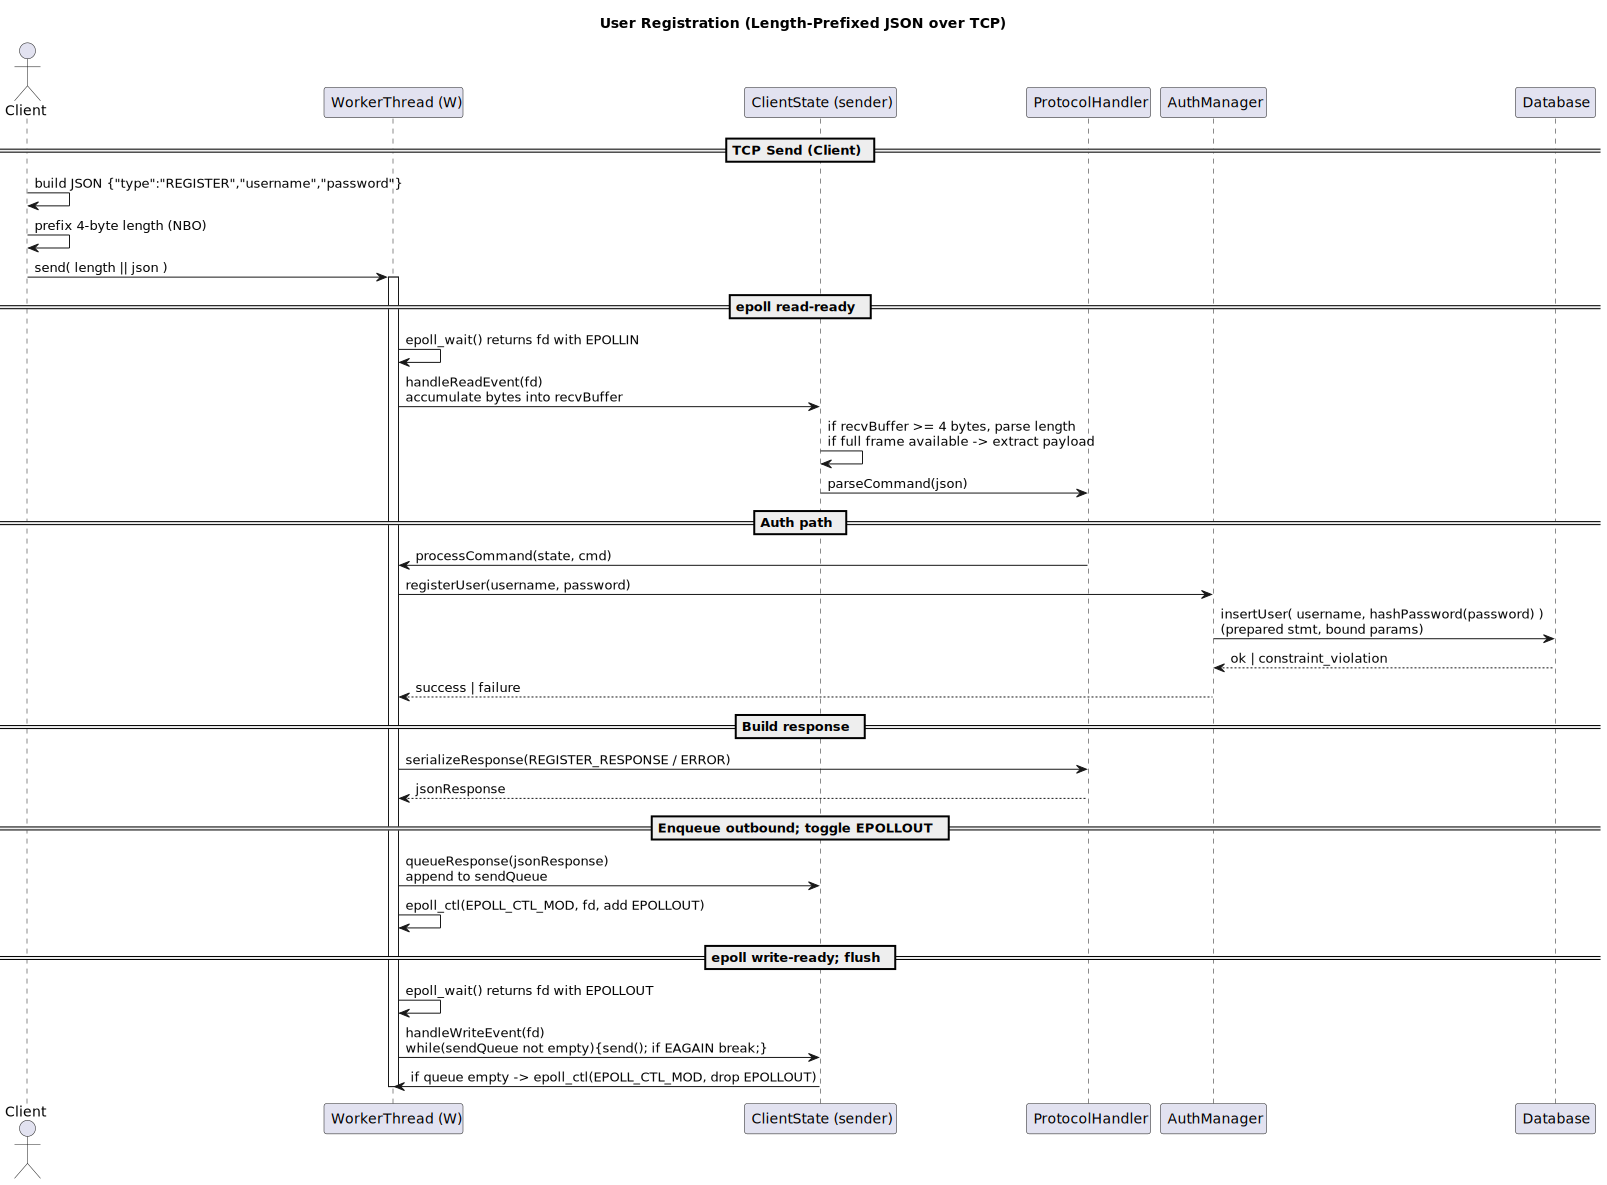
\includegraphics[width=\textwidth]{images/design_userRegister.png}
    \caption{Sequence diagram: User Registration}
    \label{fig:seq_register}
\end{figure}

\subsubsection{User Login Sequence}
Figure~\ref{fig:seq_login} shows the login process. On successful authentication, 
the client is registered in the \texttt{activeClients} map of the MessageRouter, enabling immediate routing of future messages. 
The sequence also highlights the use of per-thread SQLite handles (WAL mode) and the enqueueing of a \texttt{LOGIN\_RESPONSE} JSON frame 
for asynchronous flushing by the WorkerThread.

\begin{figure}[H]
    \centering
    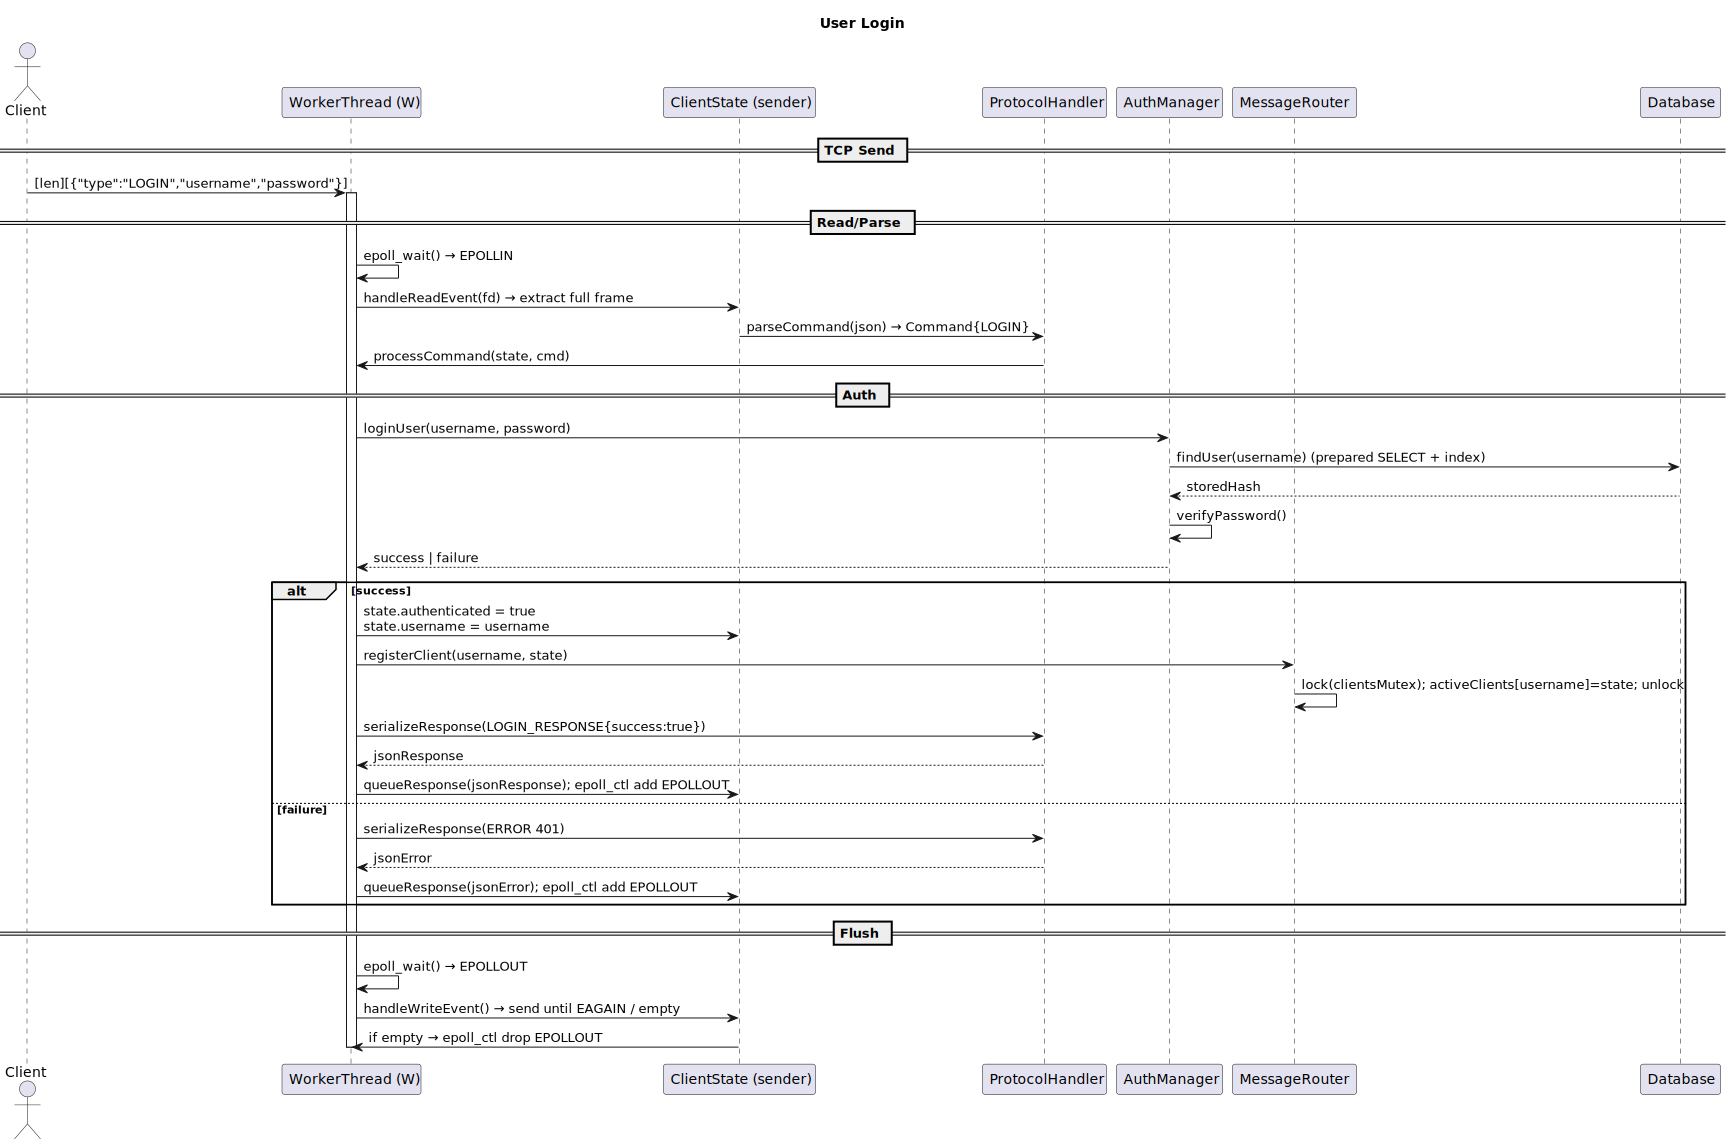
\includegraphics[width=\textwidth]{images/design_userLogin.png}
    \caption{Sequence diagram: User Login}
    \label{fig:seq_login}
\end{figure}

\subsubsection{Send Message Sequence}
Figure~\ref{fig:seq_send} models the workflow when a client issues a \texttt{SEND\_MESSAGE} command. 
The WorkerThread parses and dispatches the command to the MessageRouter, which encrypts and persists the message. 
Two alternative flows exist:
\begin{itemize}
    \item \textbf{Recipient Online:} The recipient's \texttt{ClientState} is found in \texttt{activeClients}, the message is enqueued to its sendQueue, and EPOLLOUT is enabled on the recipient's WorkerThread for immediate delivery. 
    \item \textbf{Recipient Offline:} The message remains persisted with \texttt{delivered=false}, to be flushed later when the recipient reconnects.
\end{itemize}
In both cases, the sender receives a \texttt{SEND\_MESSAGE\_RESPONSE} indicating success and delivery status.

\begin{figure}[H]
    \centering
    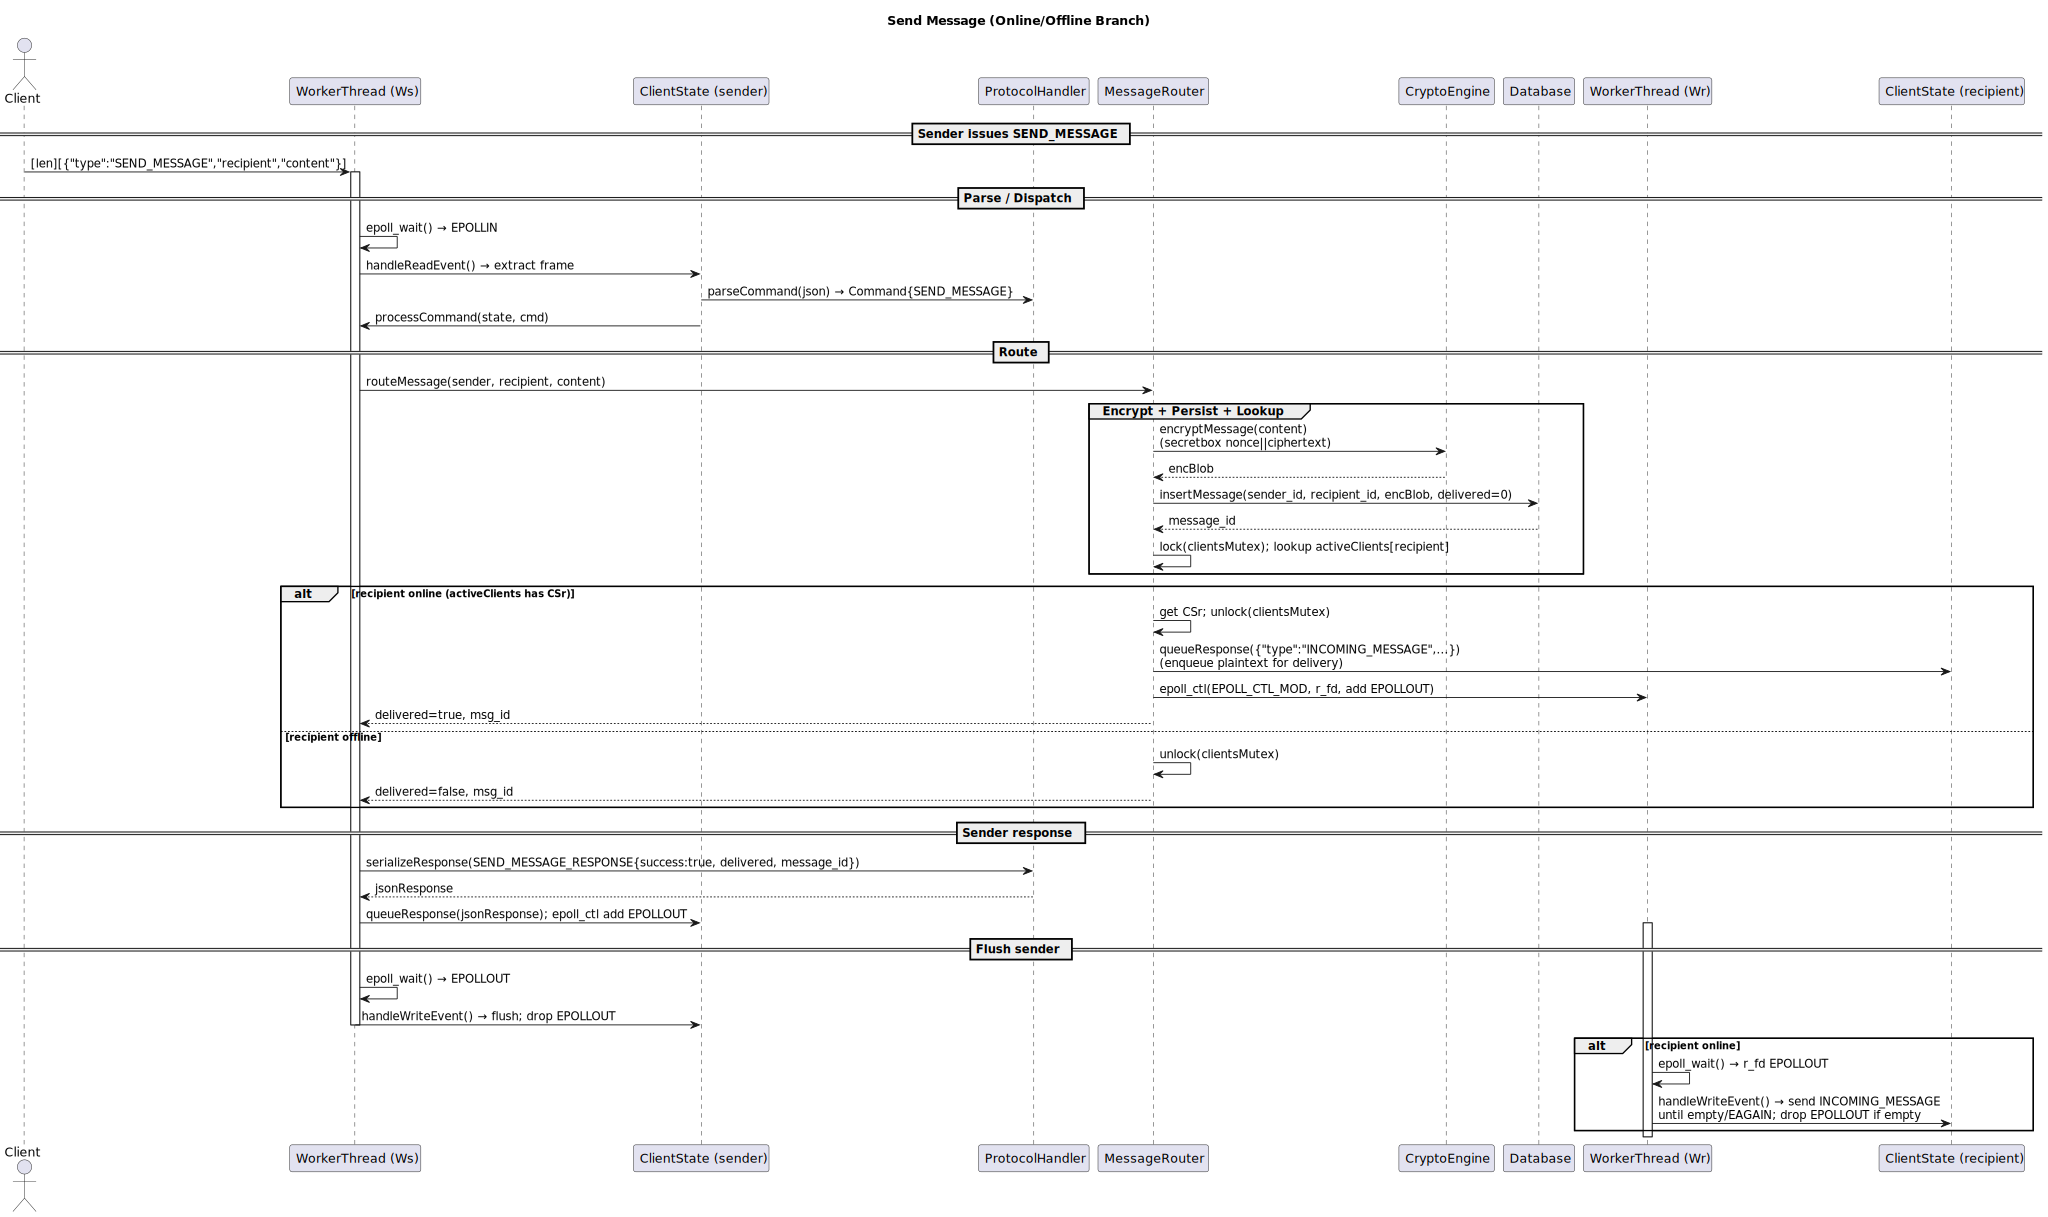
\includegraphics[width=\textwidth]{images/design_userSend.png}
    \caption{Sequence diagram: Send Message (online/offline recipient)}
    \label{fig:seq_send}
\end{figure}

\subsubsection{Message Delivery on Reconnect}
Figure~\ref{fig:seq_flush} shows the recovery of undelivered messages after a successful login. 
The WorkerThread enqueues a \texttt{LOGIN\_RESPONSE} followed by all undelivered messages retrieved from the Database, 
batched in the same sendQueue. The epoll dispatcher then flushes the entire queue asynchronously, 
marking messages as delivered once they are fully written into the kernel buffer. 
This ensures at-least-once delivery semantics while preserving ordering. 

\begin{figure}[H]
    \centering
    \includegraphics[width=\textwidth]{images/design_queueFlush.png}
    \caption{Sequence diagram: Message Delivery on Reconnect (queue flush)}
    \label{fig:seq_flush}
\end{figure}

\subsection{API Specification}
This section defines the external communication protocol used between clients and the server.
The interface is intentionally minimal yet robust—optimized for clarity, forward compatibility, and suitability for embedded deployments.

Communication occurs over persistent TCP sockets, using a lightweight binary framing layer that encapsulates UTF-8 JSON payloads.
The goal is to maintain message boundary integrity while retaining human-readable semantics.

\subsubsection{Client–Server Protocol}
All application data is transmitted as discrete binary frames, each prefixed with a 4-byte length field in network byte order (NBO).
This approach guarantees atomic message boundaries over TCP’s continuous byte stream, enabling efficient I/O multiplexing under \texttt{epoll}.

Figure~\ref{fig:protocol_specification} depicts the framing structure used for all client–server exchanges.

\begin{figure}[H]
    \centering
    \includegraphics[width=\textwidth]{images/design-Protocol_Specification.png}
    \caption{Client–server frame structure and protocol flow}
    \label{fig:protocol_specification}
\end{figure}

\noindent\textbf{Frame Format}
\begin{verbatim}
[4-byte length (network byte order)][JSON payload]
\end{verbatim}

\noindent Each frame therefore consists of:
\begin{itemize}
    \item A 32-bit unsigned integer representing the size of the following JSON document, encoded in big-endian order.
    \item A UTF-8 encoded JSON message whose structure is defined below.
\end{itemize}

\noindent\textbf{Sender Example:}
\begin{lstlisting}[language=C]
char json[] = "{\"type\":\"LOGIN\",\"username\":\"alice\",\"password\":\"secret123\"}";
uint32_t len = htonl(strlen(json));
send(sock, &len, sizeof(len), 0);   // prefix
send(sock, json, strlen(json), 0);  // payload
\end{lstlisting}

\noindent\textbf{Receiver Example:}
\begin{lstlisting}[language=C]
uint32_t len;
recv_all(sock, &len, sizeof(len));  // blocking until 4 bytes read
len = ntohl(len);
char* buffer = malloc(len);
recv_all(sock, buffer, len);        // read complete JSON payload
\end{lstlisting}

TCP may fragment transmissions arbitrarily, so the receiver must perform length-aware accumulation (\texttt{recv\_all}) until the entire frame is assembled.
This ensures predictable deserialization and safe preallocation of message buffers.

\subsubsection{Message Format (JSON)}
Each JSON message contains a mandatory \texttt{type} field identifying the operation, followed by type-specific fields.
All messages are UTF-8 encoded, newline-free, and bounded by the length prefix above.

\subsubsection*{Registration Request}
\begin{lstlisting}[language=json]
{ "type": "REGISTER", "username": "alice", "password": "secret123" }
\end{lstlisting}

\subsubsection*{Registration Response}
\begin{lstlisting}[language=json]
{ "type": "REGISTER_RESPONSE", "success": true, "user_id": 1 }
\end{lstlisting}

On error:
\begin{lstlisting}[language=json]
{ "type": "ERROR", "code": 409, "message": "Username already exists" }
\end{lstlisting}

\subsubsection*{Login Request}
\begin{lstlisting}[language=json]
{ "type": "LOGIN", "username": "alice", "password": "secret123" }
\end{lstlisting}

\subsubsection*{Login Response}
\begin{lstlisting}[language=json]
{ "type": "LOGIN_RESPONSE", "success": true }
\end{lstlisting}

\subsubsection*{Send Message Request}
\begin{lstlisting}[language=json]
{ "type": "SEND_MESSAGE", "recipient": "bob", "content": "Hello Bob!" }
\end{lstlisting}

\subsubsection*{Send Message Response}
\begin{lstlisting}[language=json]
{ "type": "SEND_MESSAGE_RESPONSE", "success": true, 
  "delivered": true, "message_id": 42 }
\end{lstlisting}

\subsubsection*{Incoming Message (server → client)}
\begin{lstlisting}[language=json]
{ "type": "INCOMING_MESSAGE", "sender": "alice", 
  "content": "Hello Bob!", "timestamp": "2025-10-15T14:30:00Z" }
\end{lstlisting}

\subsubsection*{Logout}
\begin{lstlisting}[language=json]
{ "type": "LOGOUT" }
\end{lstlisting}

\subsubsection*{Timeout (server → client)}
\begin{lstlisting}[language=json]
{ "type": "TIMEOUT", "message": "Session expired" }
\end{lstlisting}

\subsubsection{Error Codes and Semantics}
All errors are reported using a dedicated \texttt{ERROR} frame, aligned with familiar HTTP-style codes:

\begin{lstlisting}[language=json]
{ "type": "ERROR", "code": 401, "message": "Unauthorized" }
\end{lstlisting}

\begin{table}[H]
\centering
\begin{tabular}{|l|l|}
\hline
\textbf{Code} & \textbf{Meaning} \\
\hline
400 & Bad Request (malformed JSON or frame length mismatch) \\
401 & Unauthorized (invalid credentials or unauthenticated command) \\
404 & Not Found (user does not exist) \\
409 & Conflict (duplicate username on registration) \\
500 & Internal Server Error (database or runtime failure) \\
\hline
\end{tabular}
\caption{Error codes used in protocol responses}
\end{table}

Error messages are non-fatal; clients may continue communication after handling an error unless the server closes the socket.

\subsubsection{Extensibility and Forward Compatibility}
The protocol is explicitly version-resilient.  
Every message includes a mandatory \texttt{type} field, allowing clients to ignore unknown message types gracefully.  
This permits incremental feature rollout without disrupting existing deployments.

Possible future extensions include:
\begin{itemize}
    \item \textbf{Group Messaging:} \texttt{SEND\_GROUP} with an array of recipients.
    \item \textbf{Read Receipts:} \texttt{READ\_RECEIPT} acknowledging message visibility at application level.
    \item \textbf{Presence Updates:} \texttt{USER\_STATUS} broadcasts indicating online/offline states.
\end{itemize}

The binary framing remains stable across versions, ensuring backward compatibility.  
This separation of \textbf{transport framing} (binary length-prefix) from \textbf{semantic content} (JSON message schema)
allows the API to evolve safely while preserving interoperability with legacy clients.

\subsection{Graphical User Interface (UI)}
The UI will be designed to provide a user-friendly experience for interacting with the messaging protocol. Key features include:
\begin{itemize}
    \item \textbf{Login/Registration Screen:} Simple forms for user authentication and account registration.
    \item \textbf{Chat Window:} Text input area with send button and emoji support, shows past messages.
    \item \textbf{Inbox View:} List of received messages with sender, content, and timestamp.
    \item \textbf{Notifications:} Include notification alerts for incoming messages.
\end{itemize}

% Implement with either tkinter or in Figma?
% For rapid prototyping, Figma is recommended for UI design, allowing for easy iteration and feedback.
% Now, let's show the images and describe login and message
\subsubsection{Login/Registration Screen}
The login/registration screen feature input fields for username and password, along with buttons for submitting the information. See Figure~\ref{fig:login_registration_screen} for a preview of the design.
Error messages will be displayed for invalid credentials or registration issues.

\begin{figure}[H]
    \centering
    \includegraphics[width=5cm]{images/design-login.png}
    \includegraphics[width=5cm]{images/design-register.png}
    \caption{Login and Registration Screens}
    \label{fig:login_registration_screen}
\end{figure}

\subsubsection{Inbox View}
The Inbox screen will display a list of all registered users, showing the person's name, online status, ordered by last active time. See Figure~\ref{fig:chat_list_screen} for a preview of the design.

\begin{figure}[H]
    \centering
    \includegraphics[width=5cm]{images/design-chat_list.png}
    \caption{Inbox View}
    \label{fig:chat_list_screen}
\end{figure}

\subsubsection{Chat Window}
Each Chat Window (one for each recipient) provides a text input area for composing new messages, along with a send button. See Figure~\ref{fig:message_screen} for a preview of the design.

\begin{figure}[H]
    \centering
    \includegraphics[width=5cm]{images/design-chat.png}
    \caption{Chat Window}
    \label{fig:message_screen}
\end{figure}

The UI can be implemented using a cross-platform framework such as Tkinter or PyQt to ensure compatibility across different operating systems. As per listed in the non-functional requirements, the design prioritizes simplicity and ease of use, focusing on user-friendliness and the core messaging experience.

\subsection{Minimal Client Application Design (CLI)}
    % 4.9.1 Architecture
    % 4.9.2 Component Descriptions 
    % 4.9.3 Concurrency Test Cases (25 clients, race conditions)
    % 4.9.4 Security Test Cases (SQL injection, brute force)

To validate the server implementation and demonstrate end-to-end functionality, a minimal command-line client is designed.

\subsubsection{Architecture}
The client follows a simple three-layer architecture:

\begin{itemize}
    \item \textbf{Main Loop:} Parse user commands from stdin, display server responses to stdout
    \item \textbf{MessageClient:} High-level API wrapping protocol operations (register, login, send\_message)
    \item \textbf{ProtocolClient:} Socket wrapper handling length-prefixed JSON framing
\end{itemize}

Python 3.11 is chosen for rapid prototyping, built-in JSON support, and overall easier development with cross-platform compatibility.

\subsubsection{Component Descriptions}

\textbf{ProtocolClient}
\begin{itemize}
    \item \textbf{Responsibility:} Manage TCP socket, implement protocol framing
    \item \textbf{Methods:}
        \begin{itemize}
            \item \texttt{connect(host, port)}: Establish TCP connection to server
            \item \texttt{send\_command(dict)}: Serialize JSON, prepend 4-byte length, send
            \item \texttt{recv\_response()}: Read 4-byte length, read exact payload, deserialize JSON
        \end{itemize}
\end{itemize}

\textbf{MessageClient}
\begin{itemize}
    \item \textbf{Responsibility:} High-level messaging operations, session state
    \item \textbf{Attributes:}
        \begin{itemize}
            \item \texttt{protocol}: ProtocolClient instance
            \item \texttt{username}: Current authenticated user (None if logged out)
        \end{itemize}
    \item \textbf{Methods:}
        \begin{itemize}
            \item \texttt{register(username, password)}: Send REGISTER command
            \item \texttt{login(username, password)}: Send LOGIN, store username on success
            \item \texttt{send\_message(recipient, content)}: Send SEND\_MESSAGE command
            \item \texttt{logout()}: Send LOGOUT, clear username
        \end{itemize}
\end{itemize}

\subsubsection{User Interface}
Command-line interface with slash commands:
\begin{verbatim}
Available commands:
/register <username> <password>   - Create new account
/login <username> <password>      - Authenticate
/send <recipient> <message>       - Send message to user
/logout                           - End session
/quit                             - Exit client
\end{verbatim}

Example session:
\begin{verbatim}
$ python client.py localhost 8080
> /register alice secret123
[SUCCESS] User registered
> /login alice secret123
[SUCCESS] Logged in as alice
> /send bob Hello from alice!
[SUCCESS] Message sent (delivered: true)
> /logout
[SUCCESS] Logged out
\end{verbatim}

\subsubsection{Implementation Scope}
\begin{itemize}
    \item \textbf{Dependencies:} Python standard library (socket, json, struct)
    \item \textbf{Threading:} Single-threaded, blocking I/O (sufficient for an interactive demo)
    \item \textbf{Error Handling:} Parse server error codes, display user-friendly messages
\end{itemize}

\subsubsection{Design Rationale}
\begin{itemize}
    \item \textbf{Why CLI:} Faster implementation, easier debugging, shifts focus to checking protocol correctness
    \item \textbf{Why Python:} Faster prototyping and support, JSON parsing is built-in
    \item \textbf{Why single-threaded:} Client is interactive (waits for user input), no need for async complexity
    \item \textbf{Extensibility:} Architecture supports adding background message receiver thread in future
\end{itemize}

This client serves as a testing tool during development and a reference implementation for third-party client developers.
\subsubsection*{Testing Role}
Beyond serving as a demonstration client, the CLI doubles as a lightweight test harness. 
By running multiple instances in parallel, it emulates concurrent users, validates 
synchronization under load (\textit{stress tests}), and attempts malformed inputs (\textit{security tests}) to verify if the application meets its criteria. 

\subsection{Test Cases} 
    % 4.9.1 Unit Test Cases (per class/function)
    % 4.9.2 Integration Test Cases (end-to-end flows)
    % 4.9.3 Concurrency Test Cases (25 clients, race conditions)
    % 4.9.4 Security Test Cases (SQL injection, brute force)
% 4.9. Test Cases
A good design according to the Waterfall model must not only detail the application's mechanisms and policies; it must also specify how to test the application itself. We define test cases across 
four categories: \textbf{unit}, \textbf{integration}, \textbf{concurrency}, and \textbf{security}. 


\subsubsection{Unit Tests}
Unit tests validate correctness of individual classes and methods in isolation:
\begin{itemize}
    \item \textbf{AuthManager:} verify \texttt{registerUser()} rejects duplicate usernames; 
    verify \texttt{loginUser()} only succeeds with correct password.
    \item \textbf{MessageRouter:} check that \texttt{routeMessage()} queues messages for 
    offline users and immediately delivers to online ones.
    \item \textbf{Database:} test each prepared statement (INSERT, SELECT, UPDATE) with 
    mock data to confirm correct persistence and retrieval.
    \item \textbf{CryptoEngine:} ensure that encrypt→decrypt roundtrip returns identical 
    plaintext; corrupted ciphertext must fail verification.
\end{itemize}

\subsubsection{Integration Tests}
Integration tests validate end-to-end flows across multiple subsystems:
\begin{verbatim}
Test: End-to-End Message Delivery
Setup:
  1. Register users: alice, bob
  2. Login both users
Action:
  alice sends "Hello" to bob
Verify:
  1. bob receives message within 10 ms
  2. Database row shows delivered=true
  3. No memory leaks (valgrind memcheck)
\end{verbatim}

\subsubsection{Concurrency Tests}
Concurrency tests validate correct synchronization under load:
\begin{verbatim}
Test: ActiveClients Map Safety
Setup:
  Thread1: unregisterClient("alice")
  Thread2: unregisterClient("bob")
Action:
  Run both 10,000 times concurrently
Verify:
  No segmentation faults, deadlocks, or memory leaks
  Validation: valgrind --tool=helgrind
\end{verbatim}

\begin{verbatim}
Test: SQLite WAL Concurrency
Setup:
  10 threads: SELECT FROM users
  10 threads: INSERT INTO messages
  5 threads : SELECT FROM messages
Action:
  Run all concurrently
Verify:
  WAL mode scales (time << sequential baseline)
\end{verbatim}

\begin{verbatim}
Test: 25 Concurrent Logins
Setup: Pre-register 25 users
Action: Spawn 25 client threads, login simultaneously
Expected: All succeed within 2 seconds
\end{verbatim}

\subsubsection{Security Tests}
Security tests emulate malicious inputs:
\begin{itemize}
    \item \textbf{SQL Injection:} send \texttt{username="admin'; DROP TABLE users; --"} 
    → verify entry stored literally, database not modified.
    \item \textbf{Brute Force:} attempt 1000 password guesses against a test account. 
    Verify Argon2id runtime (64 MB RAM, 2 iterations) throttles throughput 
    (<50 guesses/sec on Raspberry Pi 4).
\end{itemize}

\subsection{Error Handling Strategy} 
In embedded client-server systems, robustness depends on anticipating failure conditions 
and defining deterministic recovery strategies. Errors are classified by severity, with 
clear policies for containment, recovery, and reporting. Logging complements recovery by 
providing traceability for debugging, profiling, and security auditing.

\subsubsection{Error Classification}
Errors are categorized into four severity levels, aligned with the logging subsystem:
\begin{itemize}
    \item \textbf{Critical:} Fatal conditions that prevent operation. 
    Examples: database corruption, port bind failure. 
    Action: immediate shutdown and restart attempt.
    \item \textbf{Error:} Recoverable but disruptive conditions. 
    Examples: authentication failure, message delivery timeout, database busy after retries. 
    Action: notify user via error code, log entry at \texttt{ERROR}.
    \item \textbf{Warning:} Non-fatal anomalies that may degrade performance. 
    Examples: high memory usage, slow queries, repeated failed logins. 
    Action: alert user/admin, system continues operation.
    \item \textbf{Info:} Normal events relevant for auditing. 
    Examples: user login/logout, message sent, client disconnected cleanly. 
    Action: recorded for traceability, no operator intervention.
\end{itemize}

\subsubsection{Recovery Mechanisms}
Recovery policies define consistent responses for each failure mode:
\begin{itemize}
    \item \textbf{Critical errors:} 
    Port bind failure $\rightarrow$ retry with exponential backoff. 
    Database corruption $\rightarrow$ attempt restore from backup; if persistent, shutdown.
    \item \textbf{Database lock timeout (SQLITE\_BUSY):} 
    Retry query with exponential backoff (max 10 retries). 
    If still blocked, return timeout error to client.
    \item \textbf{Worker thread crash:} 
    Detected via watchdog thread monitoring worker liveness. 
    Restart crashed worker; reassign its clients to other workers.
    \item \textbf{Client disconnect:} 
    Remove entry from \texttt{activeClients}, close socket, release buffers.
    \item \textbf{Memory exhaustion:} 
    Reject new connections with server-busy error (503 equivalent). 
    Existing clients remain unaffected.
\end{itemize}

\subsubsection{Logging Strategy}
The server maintains structured logs to support both debugging and audit trails.
Logs are categorized by severity using the following enum:
\begin{verbatim}
enum LogLevel { DEBUG, INFO, WARNING, ERROR, CRITICAL };
\end{verbatim}

\textbf{Examples by level:}
\begin{verbatim}
DEBUG:    "Thread 4 processing message ID 123"
INFO:     "User alice logged in from 192.168.1.100"
WARNING:  "Failed login attempt for user eve (3rd attempt in 10s)"
ERROR:    "Database query failed: SQLITE_BUSY after 10 retries"
CRITICAL: "Cannot bind to port 8080, exiting"
\end{verbatim}

\textbf{Rotation Policy:} 
To mitigate microSD wear and database growth, logs are periodically pruned:
\begin{verbatim}
if (log_count > 10000) {
    DELETE FROM logs 
    WHERE id < (SELECT MAX(id) - 5000 FROM logs);
}
\end{verbatim}
Alternatively, logs can be offloaded to external syslog or exported for offline analysis. 

This layered strategy ensures that errors are detected, isolated, and either recovered 
or escalated, while maintaining full visibility into system operation.

The following table resumes the error types, and the corresponding system response and error logging. 
\begin{table}[H]
\centering
\begin{tabular}{|l|l|l|}
\hline
\textbf{Error Type} & \textbf{System Response} & \textbf{Log Level} \\
\hline
Port bind failure         & Retry with backoff, shutdown if persistent & CRITICAL \\
Database corruption       & Attempt restore, shutdown if unrecoverable & CRITICAL \\
Database lock timeout     & Retry (max 10), return timeout to client   & ERROR \\
Worker thread crash       & Respawn worker, reassign clients           & ERROR \\
Client disconnect         & Cleanup state, unregister client           & INFO \\
Message delivery timeout  & Notify client, log failure                 & ERROR \\
High memory usage         & Alert admin, continue operation            & WARNING \\
Repeated failed logins    & Log attempt, possible rate limit           & WARNING \\
Normal login/logout       & Record event                               & INFO \\
Message sent              & Record event                               & INFO \\
\hline
\end{tabular}
\caption{Error classification matrix: mapping failure modes to recovery actions and log levels}
\end{table}

\subsection{Dry Run Tables}

\begin{table}[H]
\centering
\caption{Dry Run Table (Authentication Flow) — User ``alice'' logs in with password ``secret123''}
\scriptsize
\begin{tabular}{>{\scriptsize}c >{\scriptsize}c >{\scriptsize\ttfamily}p{5.5cm} >{\scriptsize}p{5.5cm}}
\toprule
Step & Thread & Function & Variables / Actions \\
\midrule
1  & Worker 3 & handleReadEvent(fd) & buffer = \{"type":"LOGIN","username":"alice","password":"secret123"\} \\
2  & Worker 3 & ProtocolHandler::parseCommand() & cmd.type=LOGIN, cmd.username="alice", cmd.password="secret123" \\
3  & Worker 3 & WorkerThread::processCommand() & Dispatch LOGIN → AuthManager \\
4  & Worker 3 & AuthManager::loginUser() & username="alice", pw="secret123" \\
5  & Worker 3 & Database::findUser() & SELECT password\_hash FROM users WHERE username=? \\
6  & Worker 3 & sqlite3\_step() & storedHash="\$argon2id\$..." \\
7  & Worker 3 & libsodium::crypto\_pwhash\_str\_verify() & Compare storedHash vs "secret123" → success \\
8  & Worker 3 & MessageRouter::registerClient() & lock(clientsMutex); activeClients["alice"]=state; unlock() \\
9  & Worker 3 & ClientState::queueResponse() & queue LOGIN\_RESPONSE JSON, enable EPOLLOUT \\
10 & Worker 3 & Database::getQueuedMessages() & SELECT * FROM messages WHERE recipient="alice" AND delivered=0 \\
11 & Worker 3 & sqlite3\_step() & 3 undelivered messages found \\
12 & Worker 3 & ClientState::queueResponse() & enqueue messages into sendQueue, keep EPOLLOUT enabled \\
13 & Worker 3 & handleWriteEvent(fd) & flush queue to socket until empty, disable EPOLLOUT if drained \\
\bottomrule
\end{tabular}
\end{table}

\vspace{0.4cm}

\begin{table}[H]
\centering
\caption{Dry Run Table (Message Routing Flow) — Alice sends message to Bob (Bob online)}
\scriptsize
\begin{tabular}{>{\scriptsize}c >{\scriptsize}c >{\scriptsize\ttfamily}p{4.5cm} >{\scriptsize}p{5.5cm}}
\toprule
Step & Thread & Function & Variables / Actions \\
\midrule
1  & Worker 3 & handleReadEvent(fd) & buffer=\{"type":"SEND\_MESSAGE","recipient":"bob","content":"Hello!"\} \\
2  & Worker 3 & ProtocolHandler::parseCommand() & cmd.recipient="bob", cmd.content="Hello!" \\
3  & Worker 3 & WorkerThread::processCommand() & Dispatch SEND\_MESSAGE → MessageRouter \\
4  & Worker 3 & CryptoEngine::encryptMessage() & plaintext="Hello!", output=ciphertext \\
5  & Worker 3 & Database::insertMessage() & sender=alice, recipient=bob, content=ciphertext, delivered=0 \\
6  & Worker 3 & MessageRouter::routeMessage() & lock(clientsMutex); lookup "bob" \\
7  & Worker 3 & — & activeClients["bob"] found → ClientState* on Worker 5 \\
8  & Worker 3 & unlock(clientsMutex) & — \\
9  & Worker 3 & bobState::queueResponse() & enqueue INCOMING\_MESSAGE JSON, enable EPOLLOUT on Worker 5 epollFd \\
10 & Worker 5 & handleWriteEvent(fd) & flush sendQueue to bob's socket \\
11 & Worker 5 & Database::markDelivered() & UPDATE messages SET delivered=1 WHERE id=? \\
12 & Worker 3 & aliceState::queueResponse() & enqueue SEND\_MESSAGE\_RESPONSE JSON ("delivered":true) \\
13 & Worker 3 & handleWriteEvent(fd) & flush confirmation to alice \\
\bottomrule
\end{tabular}
\end{table}

\subsection{Conclusion}
With this, we conclude the design section. We outlined the system's workings through Class Diagrams, and specified how these are to interact with flowcharts. Detailed information was provided regarding the concurrency and security mechanisms, namely how an event-guided thread-pool is to handle all the brute work of the system. We specified the API for message exchange between clients, detailed how modules integrate through concurrency and database abstractions, and outlined a basic CLI interface through which we'll test the system's mechanisms, leaving third-party client implementations for a future project.

\appendix
\section*{Appendix A — Glossary of Terms}

\begin{description}
  \item[ACID] Atomicity, Consistency, Isolation, Durability — transactional properties guaranteeing database integrity.
  \item[AEAD] Authenticated Encryption with Associated Data — cryptographic mode providing both confidentiality and integrity.
  \item[API] Application Programming Interface — external communication contract between components.
  \item[CFS] Completely Fair Scheduler — Linux default process scheduler.
  \item[CLI] Command Line Interface — text-based client front-end.
  \item[DB] Database — persistent data store; here, the DB Engine is SQLite 3.
  \item[EPOLL] Linux kernel I/O event notification facility used for non-blocking multiplexing.
  \item[FD] File Descriptor — integer handle identifying an open socket or file.
  \item[GCC] GNU Compiler Collection — used for cross-compiling ARM binaries.
  \item[GPIO] General Purpose Input/Output — digital pins on Raspberry Pi used for LED control.
  \item[MPSC] Multi-Producer Single-Consumer queue — used for connection assignment.
  \item[NBO] Network Byte Order — big-endian representation used in message length prefixes.
  \item[SQLITE WAL] Write-Ahead Logging — journaling mode enabling concurrent reads and atomic commits.
  \item[TCP] Transmission Control Protocol — reliable, ordered byte-stream transport.
  \item[TTM] Time-To-Market — time from concept to deliverable product.
  \item[TTP] Time-To-Prototype — time to reach a functional prototype.
\end{description}
